	\chapter{Ο πηρύνας της Μηχανής}
	
	Ένα framework το οποίο επεκτείνεται και διακλαδώνεται σε πολλές υπο-βιβλιοθήκες, στηρίζεται στη θεμελιώση ενός framework core, του πηρύνα της βιβλιοθήκη. Το \gls{API} του πηρύνα πρέπει να είναι εύκολο στην κατανόηση, να αποτελείται από αυτοεπεξηγούμενες αφαιρέσεις, οι οποίες εκθέτουν μόνο τα απολύτος απαραίτητα, ώστε οι υποβιβλιοθήκες που χρησιμοποιούν τον πηρύνα να μην δεσμεύονται σε υλοποιήσεις, να περιορίζει σε συγκεκριμένο pipeline χρήσης για αποφυγή απρόβλεπτων συμπεριφορών και να προσφέρει δυνατότητες επεκτασιμότητας.  \cite{jaroslav08} Ο πηρύνας περιέχει υποσυστήματα τα οποία μπορούν να χρησιμοποιηθούν τη δημιουργία πολλών είδων παιχνιδιών.
		
	\section{Κύκλος ζωής πηρύνα}	
	Κάθε οντότητα από τη στιγμή της δημιουργίας της στο περιβάλλον της μηχανής μέχρι την καταστροφής της και διαγραφή της από την μνήμη, περνά από κάποια προκαθορισμένα στάδια τα οποία εκτελούνται ανάλογα με την κατάσταση του υλικού και του λογισμικού.
	
	\begin{itemize}
		\item Initialization εκτελείται μόνο κατά τη δημιουργία
		\item Game loop εκτελείται συνέχεια σε βρόγχο
		\item Disposing εκτελείται κατά την καταστροφή
	\end{itemize}
	
	\begin{figure}[h!]
		\centering
		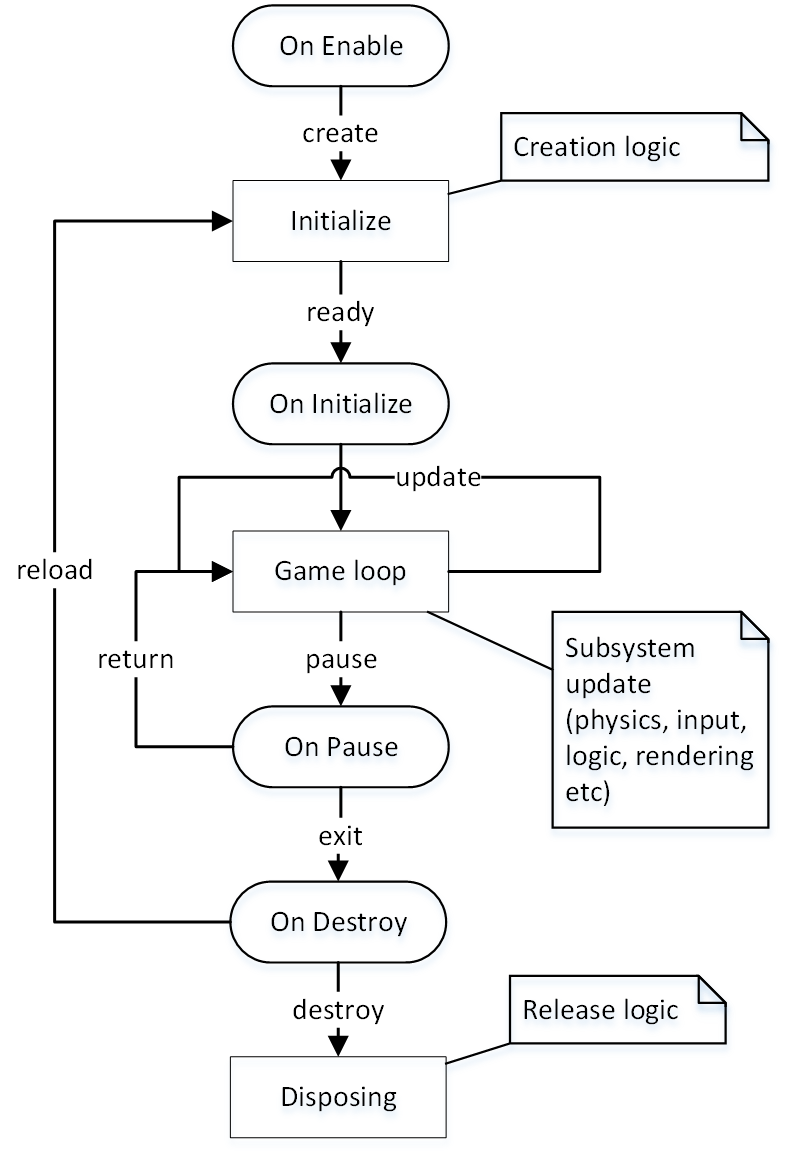
\includegraphics[width=80mm]{Images/core_lifecycle}
		\caption{Core Lifecycle}
		\label{fig:corelifecycle}
	\end{figure}
		
	\subsection{Game Loop}
	To game loop εγκυάται τη συνεπής ενημέρωση των υποσυστημάτων ανάλογα με το προκαθορισμένο χρονικό βήμα. Χωρίς το ανεξάρτητο σύστημα ενημέρωσης υποσυστημάτων, η ενημέρωση θα γινόταν στον κύκλο εκτέλεσης του επεξεργαστή με αποτέλεσμα την διαφορετική εμπειρία ανά επεξεργαστή και μηχάνημα.
	
	Το κάθε υποσύστημα έχει διαφορετικές απαιτήσεις για τη βέλτιστη λειτουργία. Το collision detection system μπορεί να χρειάζεται να ενημερώνεται εκατό φορές το δευτερόλεπτο, ενώ το σύστημα τεχνητής νοημοσύνης δύο φορές το δευτερόλεπτο. Η πιο συνηθισμένη τεχνική είναι να υπάρχουν δύο κύρια update loops
	\begin{itemize}
	\item το game loop στο οποίο ενημερώνονται όλα τα υποσυστήματα, physics, logic, dynamics κλπ
	\item rendering loop στο οποίο γίνονται οι κλήσεις στην κάρτα γραφικών και τρέχει στα 50-60 \gls{FPS}
	\end{itemize}
	
	Η διαφορά του χρόνου μεταξύ των ενημερώσεων πρέπει να είναι εγγυημένη για παράδειγμα σε μια μηχανή στην οποία το rendering loop τρέχει στα 60 \gls{FPS} υπάρχει η συχνότητα ενημέρωσης
	\begin{equation}
	 F = 1/T =>  F = 1000ms/60 => F = 16ms. 
	\end{equation}Για να μπορεί να εγγυάται το σύστημα αυτή την αναλογία, πρέπει να μετράει τη διαφορά χρόνου μεταξύ κάθε κλήσης, να εκτελεί τον κώδικα στο συγκεκριμένο loop και για τον υπόλοιπο χρόνο το thread να κοιμάται.
	
	Στα συστήματα πραγματικού χρόνου, η έννοια της διάρκειας και του χρόνου πρέπει να χειρίζεται ως μια ξεχωριστή οντότητα. Ο χρόνος πρέπει να είναι ανεξάρτητος από τον πραγματικό χρόνο. Ένα animation το οποίο γίνεται render σε πραγματικό χρόνο, μπορεί να παίξει αντίστροφα ή με διπλάσια ταχύτητα, αν το χρονοδιάγραμμα στο οποίο ανταποκρίνεται, χειρίζεται τον χρόνο διαφορετικά.
	Όλα τα συστήματα ενημερώνονται γραμμικά συναρτήσει του χρόνου του οποίο παρέχεται ως είσοδος.
	
	\paragraph{Χρόνος}
	Στα συστήματα πραγματικού χρόνου, η έννοια της διάρκειας και του χρόνου πρέπει να χειρίζεται απομονωμένος. Ο χρόνος του παιχνιδιού  είναι ανεξάρτητος από τον πραγματικό χρόνο. Η ενημερώση και η λογική των συστημάτων γίνεται με βάση τη διαφορά χρόνου μεταξύ ενημερώσεων. Με αυτή την στρατηγική, η εμπειρία δεν διαφοροποιείται με λιγότερα \gls{FPS} και ένα animation το οποίο γίνεται render σε πραγματικό χρόνο, μπορεί να παίξει αντίστροφα ή με διπλάσια ταχύτητα, αν το χρονοδιάγραμμα στο οποίο ανταποκρίνεται, χειρίζεται τον χρόνο διαφορετικά.
	Όλα τα συστήματα ενημερώνονται γραμμικά συναρτήσει μιας αφαίρεσης η οποία περιλαμβάνει τη διαφορά χρόνου.
	\subsection{Υποσυστήματα}
	Το κάθε υποσύστημα δημιουργείται ενημερώνεται και καταστρέφεται μέσα στο γενικό κύκλο ζωής του πηρύνα. Το κάθε υποσύστημα έχει εσωτερικά το δικό του κύκλο ζωής και κύκλο ενημέρωσης ο οποίος λειτουργεί μέσα στην έκταση του εξωτερικού κύκλου ζωής.
	
	\subsection{Τεχνικές Ενημέρωσης Υποσυστημάτων}
	Τα υποσυστήματα με κάποιο τρόπο πρέπει να ενημερώνονται και να επικοινωνούν μεταξύ τους ή να στέλνουν μηνύματα όταν συμβεί κάποιο γεγονός. Υπάρχουν διάφορές τεχνικές ενημέρωσης υποσυστημάτων.
	\begin{itemize}
	\item Message Pumps: τα υποσυστήματα στέλνουν μηνύματα σε ένα message bus και τα συστήματα ενημερώνονται όταν εξυπηρετείται το μήνυμα. Παραμένουν άεργα εφόσον δεν υπάρχει μήνυμα προς εξυπηρέτηση.
	\item Call-back driven: τα υποσυστήματα παρέχουν call-back λειτουργικότητα. Δηλαδή τη δυνατότητα να θέσεις τι κώδικας θα εκτελεστεί κατά κάποιο συμβάν. Ένα συμβάν μπορεί να είναι η σύγκρουση μεταξύ δύο αντικειμένων. Ο χρήστης μπορεί να πει ότι όταν συμβεί σύγκρουση μεταξύ του παίχτη και του εχθρού, ο παίχτης θα χάσει ζωή.
	\end{itemize}
	
	\begin{figure}[h!]
		\centering
		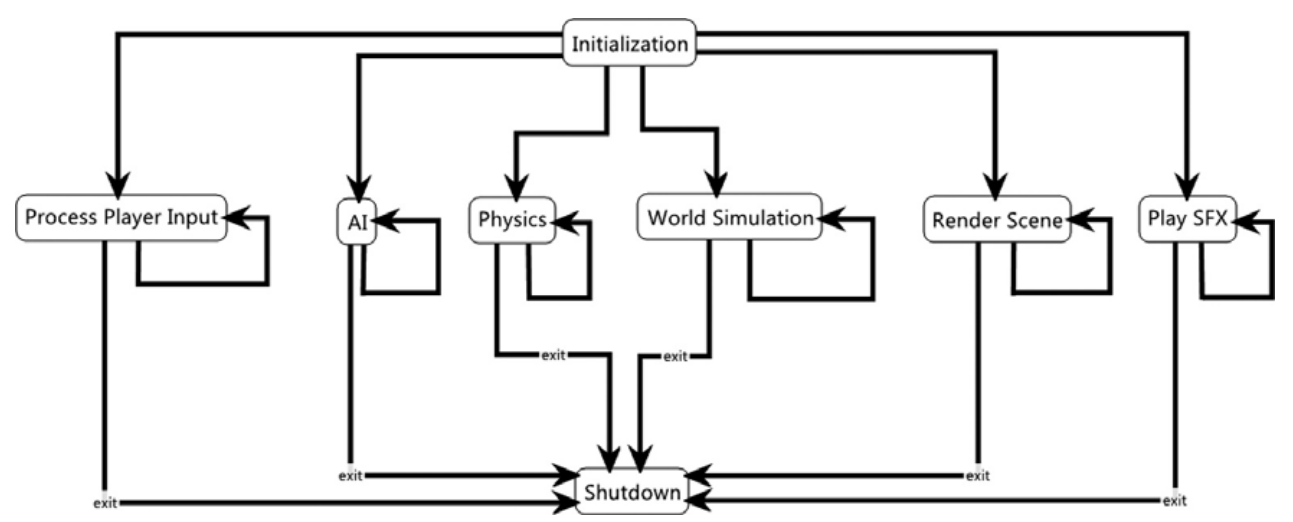
\includegraphics[width=160mm]{Images/game_coding_complete_chapter7_gameloops}
		\caption{game loops}
		\label{fig:gameloops}
	\end{figure}
		
	\section{ScreenSystem}
	Σε ένα τυπικό χρόνο εκτέλεσης ενός παιχνιδιού, το παιχνίδι περνά από διάφορες καταστάσεις. Οι καταστάσεις αυτές μπορεί να είναι η προσωρινή παύση, ένα μενού ρυθμίσεων ένα \gls{GUI} επιλογών το οποίο επικαλύπτει το τρέχον παιχνίδι ή απoδίδεται στον ίδιο render buffer. Το παιχνίδι χωρίζεται σε σκηνές, σε επίπεδα και σε χάρτες οι οποίες έχουν ξεχωριστό τρόπο απόδοσης στην οθόνη. Μία σκηνή μπορεί να αποδίδεται από διάφορες υποσκηνές οι οποίες δίνουν την ψευδαίσθηση του βάθους στο φόντο. Η σειρά απόδοσης των σκηνών πρέπει να είναι ρυθμιζόμενη και ελεγχόμενη. Η κάθε σκηνή μπορεί να παρομοιαστεί ως μια οθόνη.

	\subsection{Απαιτήσεις}
	Ο χρήστης του συστήματος έχει πλήρη έλεγχο της κάθε οθόνης-σκηνής και προσαρμόζει τη λογική και την απόδοση ανάλογα. Το κεντρικό σύστημα διαχείρισης προσφέρει τη δυνατότητα προετοιμασίας οθονών, αναζήτησης μέσω κλειδιών, αυτόματη διαχείριση και εναλλαγή και εξατομίκευση τους. Για τη διατήρηση της συνοχής κατά την εναλλαγή οθόνων, προσφέρεται η δυνατότητα εξατομίκευσης της απόδοσης κατά τις μεταβάσεις.

	\begin{figure}[h!]
		\centering
		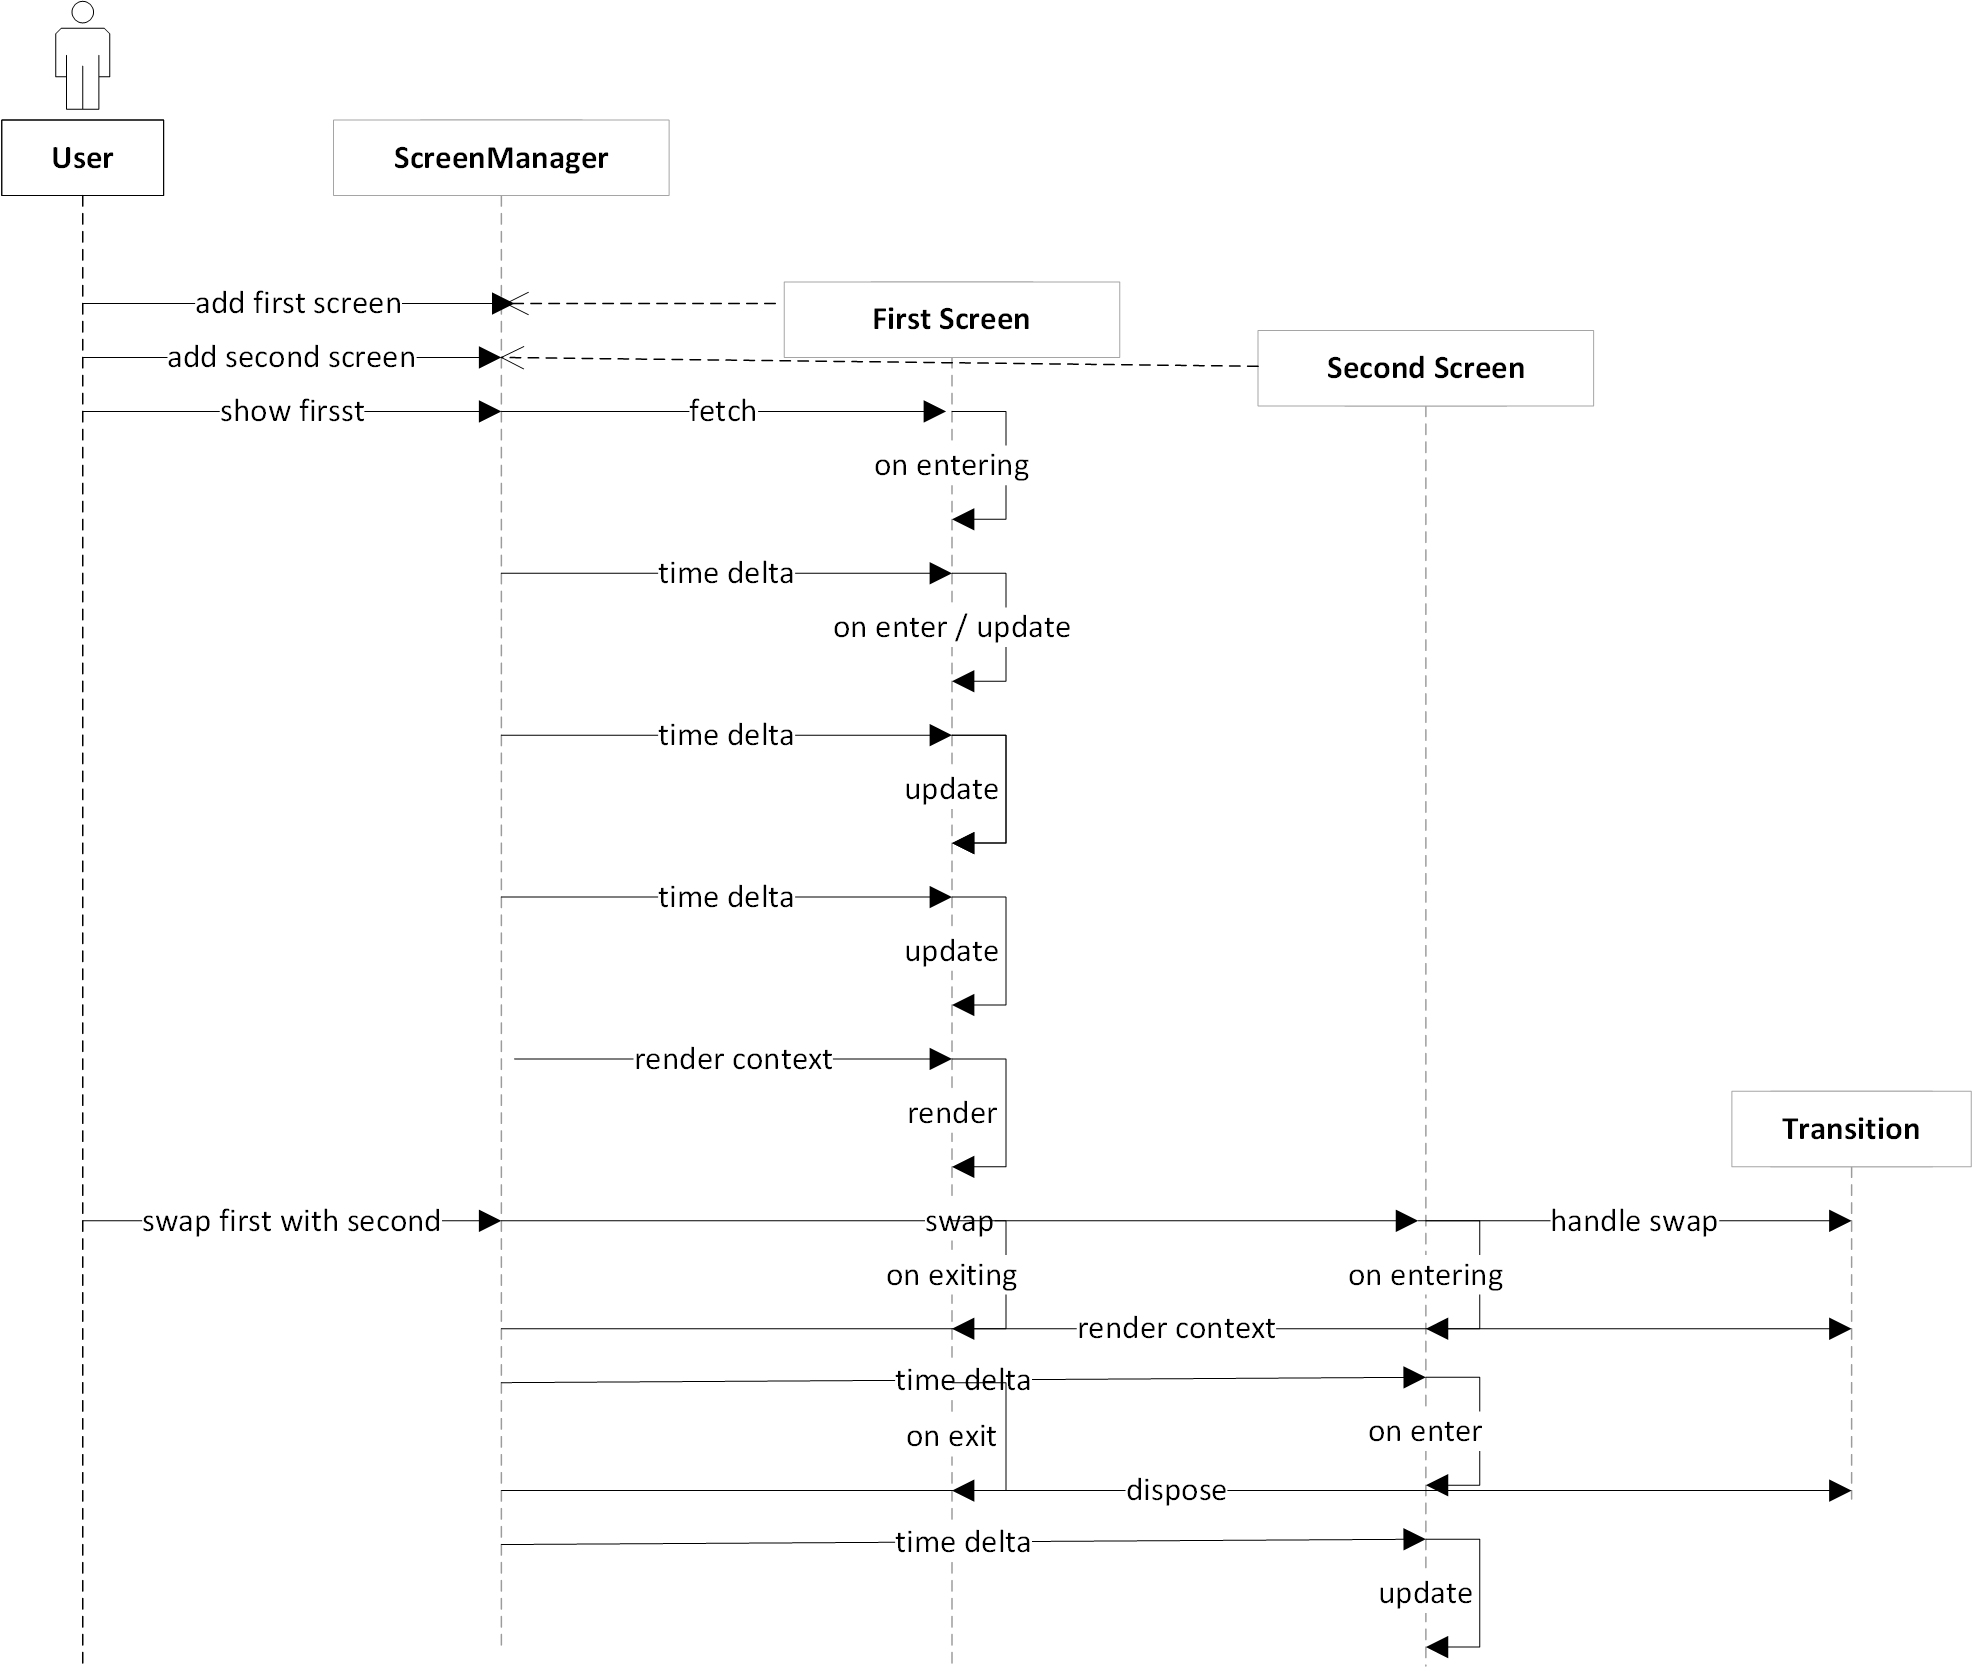
\includegraphics[width=165mm]{Images/screensystem_sequence}
		\caption{screensystem sequence}
		\label{fig:screensystem_sequence}
	\end{figure}	
	
	\subsection{Συστατικά του συστήματος}		
	\paragraph{Κεντρικό σύστημα διαχείρισης}
	Οι λειτουργίες του συστήματος.
	\begin{itemize}
	\item Απόδοση και ενημέρωσης 1-N σκηνών με δυναμικά εναλλασσόμενη σειρά στο πλαίσιο του κύκλου ζωής του πηρύνα.
	\item Προετοιμασία των οθονών και δυνατότητα εύρεσης χρησιμοποιώντας κλειδιά.
	\item Εύκολη προβολή, απόκριψη, εναλλαγή οθονών χρησιμοποιώντας κλειδιά.
	\item Δυνατότητα εξατομίκευσης της απόδοσης κατά τις διάφορες μεταβάσεις των σκηνών.
	\end{itemize}

	\paragraph{Screen host}
	\begin{itemize}
		\item Παραμετροποίηση συμβάντων κατά τις αλλαγές κατάστασης
		\item Προσαρμοσμένη λογική και απόδοση 
		\item Εντολές αλλαγής κατάστασης
		\item Εξατομίκευση απόδοσης κατά την εναλλαγή κατάστασης
	\end{itemize}
	
	\paragraph{Εναλλαγή οθονών}
	Η εξατομίκευση και παραμετροποίηση της εναλλαγής οθονών λαμβάνει μέρος μέσα στο γενικό πλαίσιο απόδοσης οθονών. Ο εξατομικευτής αναλαμβανει την απόδοση του screen buffer στον οποίο αποδόθηκε η οθόνη, την κατάσταση στην οποία βρίσκεται η οθόνη, την κατεύθυνση και το ποσοστό εξέλιξης της εναλλαγής. 
			
	\lstset
	{
		style=sharpc, 
		caption={Transition Delegate}
	}
	\begin{lstlisting}	
delegate void TransitionRenderAction(ScreenState state, float progress, RenderTarget2D renderTarget, SpriteBatch batch);
	\end{lstlisting}
	
	
	\subsection{Αρχιτεκτονική}
	\begin{figure}[h!]	
		\centering
		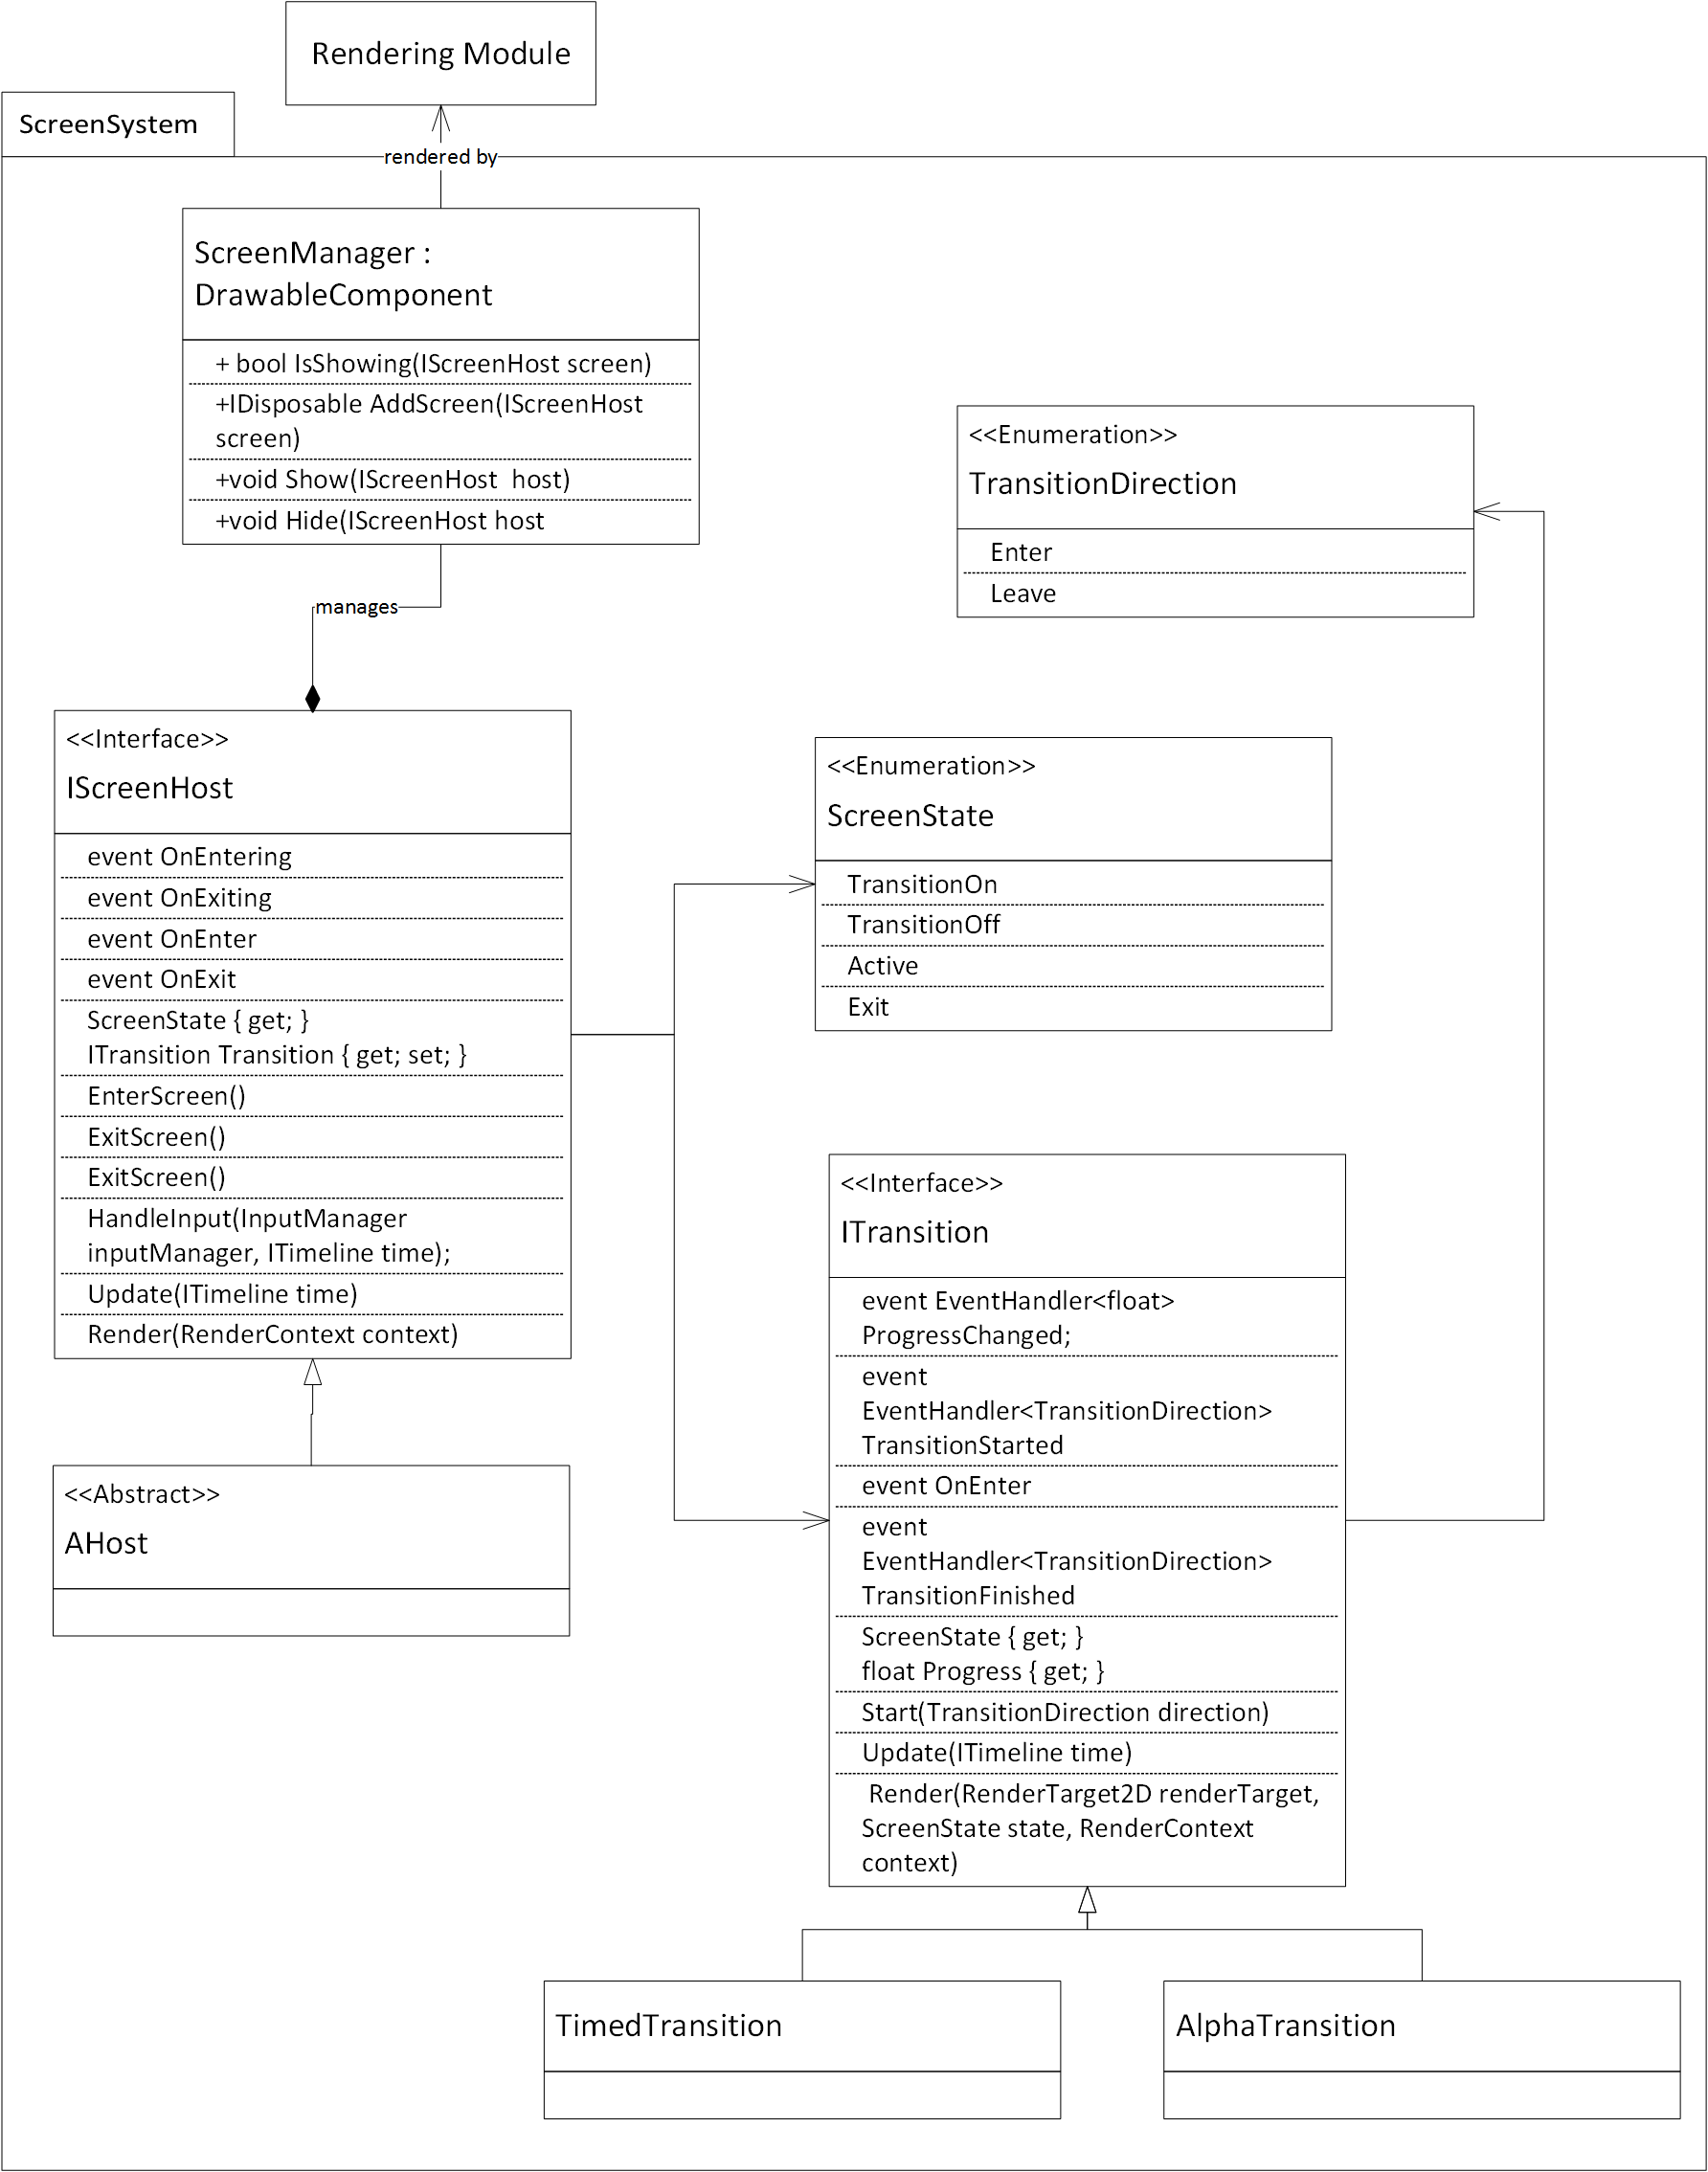
\includegraphics[width=160mm]{Images/core_screensystem}
		\caption{core screensystem}
		\label{fig:core_screensystem}
	\end{figure}		
	
	\subsection{Παράδειγματα χρήσης API}

	\lstset
	{
		style=sharpc, 
		caption={Transition Delegate}
	}
	\begin{lstlisting}
screenHost
.AddScreen(
	"FirstScreen",
	() => new MyFirstScreen());
		
screenHost["FirstScreen"]
.Show()
.Transition(
	Transition.WithTime(
         TimeSpan.FromSeconds(0.5),
         (state, progress, target, context) =>
         context.Batch.Draw(target, 
         (float)Math.Pow(progress - 1.0f, 2) * context.ScreenWidth, 
         Color.White * progress
    )
);
     
screenHost["FirstScreen"]
.Hide();   
	\end{lstlisting}
	\section{Input System}
	\subsection{Human Interface devices}
	Η μηχανή πρέπει να είναι σε θέση να διαβάζει, να επεξεργάζεται και να χρησιμοποιεί συσκευές ανθρώπινης διεπαφής. Η διαδικασία ανάγνωσης χωρίζεται στις παρακάτω κατηγορίες:
	\begin{itemize}
	\item Polling: η κατάσταση κάποιον συσκευών (κυρίως της παλιάς σχολής) διαβάζεται ρωτώντας τη συσκευή για την κατάστασή της περιοδικά. Αυτό καταλήγει σε πλεονασμό γιατί ρωτάει πολλές φορές χωρίς να παίρνει απάντηση και με μικρή καθυστέρηση γιατί η αλλαγή κατάστασης μπορεί να γίνει μεταξύ ερωτήσεων.
	\item Interrupts (διακοπές): Οι συσκευές στέλνουν δεδομένα μόνο όταν αλλάξει η κατάσταση με κάποιο τρόπο. Ο χρήστης μπορεί γράψει κώδικα και να τον εγγράψει με τρόπο ώστε να εκτελείται μόνο όταν συμβεί κάποια αλλαγή κατάστασης.
	\end{itemize}
	
	\subsection{Τύποι Input}
	
	\begin{itemize}	
	\item Digital Buttons: τα ψηφιακά κουμπιά έχουν δύο καταστάσεις: pressed / not pressed
	\item Analog axes and buttons: τα αναλογικά επιστρέφουν εύρος τιμών: το βαθμό της πίεσης της σκανδάλης ή τη θέση του μοχλού στο δισδιάστατο άξονα. 
	\item Relative Axes: οι αναφορικοί άξονες επιστρέφουν τιμές σε σχέση με το τελευταίο σημείο στο οποίο έγινε κάποια αλλαγή πχ το ποντίκι επιστρέφει τη διαφορά θέσης σε σχέση με το τελευταίο σημείο στο οποίο μετακινήθηκε.
	\item Accelerators: Ανιχνεύουν τρισδιάστατες επιταχύνσεις.
	\item Sensor bars: Αισθητήρες όπως οι κάμερες.
	\item Touch / gestures: Σε οθόνες αφής όπως στις οθόνες στα έξυπνα τηλέφωνα.
	\end{itemize}
	
	\subsection{Απαιτήσεις υποσυστήματος}
	Η οντότητα θέλει να εκτελέσει κώδικα προσανατολισμένο κατά συμβάν εισόδου από συσκευή ανθρώπινης διεπαφής. Ο κώδικας αυτός εκτελείται αντίστοιχα για keyboard-mouse και για gamepad. O χρήστης μπορεί να αλλάξει συσκευή διεπαφής ενώ βρίσκεται σε τρέχον παιχνίδι. Η βιβλιοθήκη δεν πρέπει να στηρίζεται σε κανένα υλικό ή συσκευή. Επίσης θέλει τη δυνατότητα να ακυρώνει συμβάντα.
	
	\subsection{Observers-listeners}
	Το κάθε υποσύστημα διαχείρισης συσκευών ανθρώπινων διεπαφών αποτελείται από τον διαχειριστή για παράδειγμα τον MouseListener ή Keyboard listener, το οποίο χρησιμοποιεί τις βιβλιοθήκες του τρέχον λειτουργικού για την επιστολή συμβάντων των διεπαφών. Ανάλογα με την πλατφόρμα στην οποία έγινε compile δημιουργούνται οι αντίστοιχοι listeners μέσω του abstract factory.
	Ο χρήστης μπορεί να προσκολήσει κώδικα ο οποίος να εκτελείται ανά συμβαν π.χ. στη μετακίνηση του ποντικιού.Οι listeners κατά την εισαγωγή τους, επιστρέφουν ένα αντικείμενο το οποίο μπορεί να χρησιμοποιηθεί για την κατάργησή τους. Οι listeners ανάλογα με τις συνθήκες επιστολής, όπως το δέλτα του χρόνου επιστολής συμβάντος διπλού click ειναι 200ms, αποστέλλουν τα συμβάντα στoυς καταχωρημένους εκτελεστές. Το κεντρικό σύστημα διαχείρισης εισόδου ενημερώνει όλες τις συνδεδεμένες συσκευές εισόδου. 
	Ο εκτελέσιμος κώδικας μπορεί να γραφτεί μια φορά, ανεξαρτήτως συμβάντος, και να προσκοληθεί στο initialization του lifecycle σε υποσυστήματα διεπαφών. Επίσης με τη χρήση των active binders, μπορεί να γίνει απενεργοποίηση των listeners π.χ. όταν είναι ανοιχτό το menu επιλογών, οι o ActiveBinder του παιχνιδιού είναι απενεργοποιημένος, με αποτέλεσμα τα συμβάτα τα οποία είναι προσκολλημένα στον InputManager να μην εκτελούνται.
	
	\begin{figure}[h!]
		\centering
		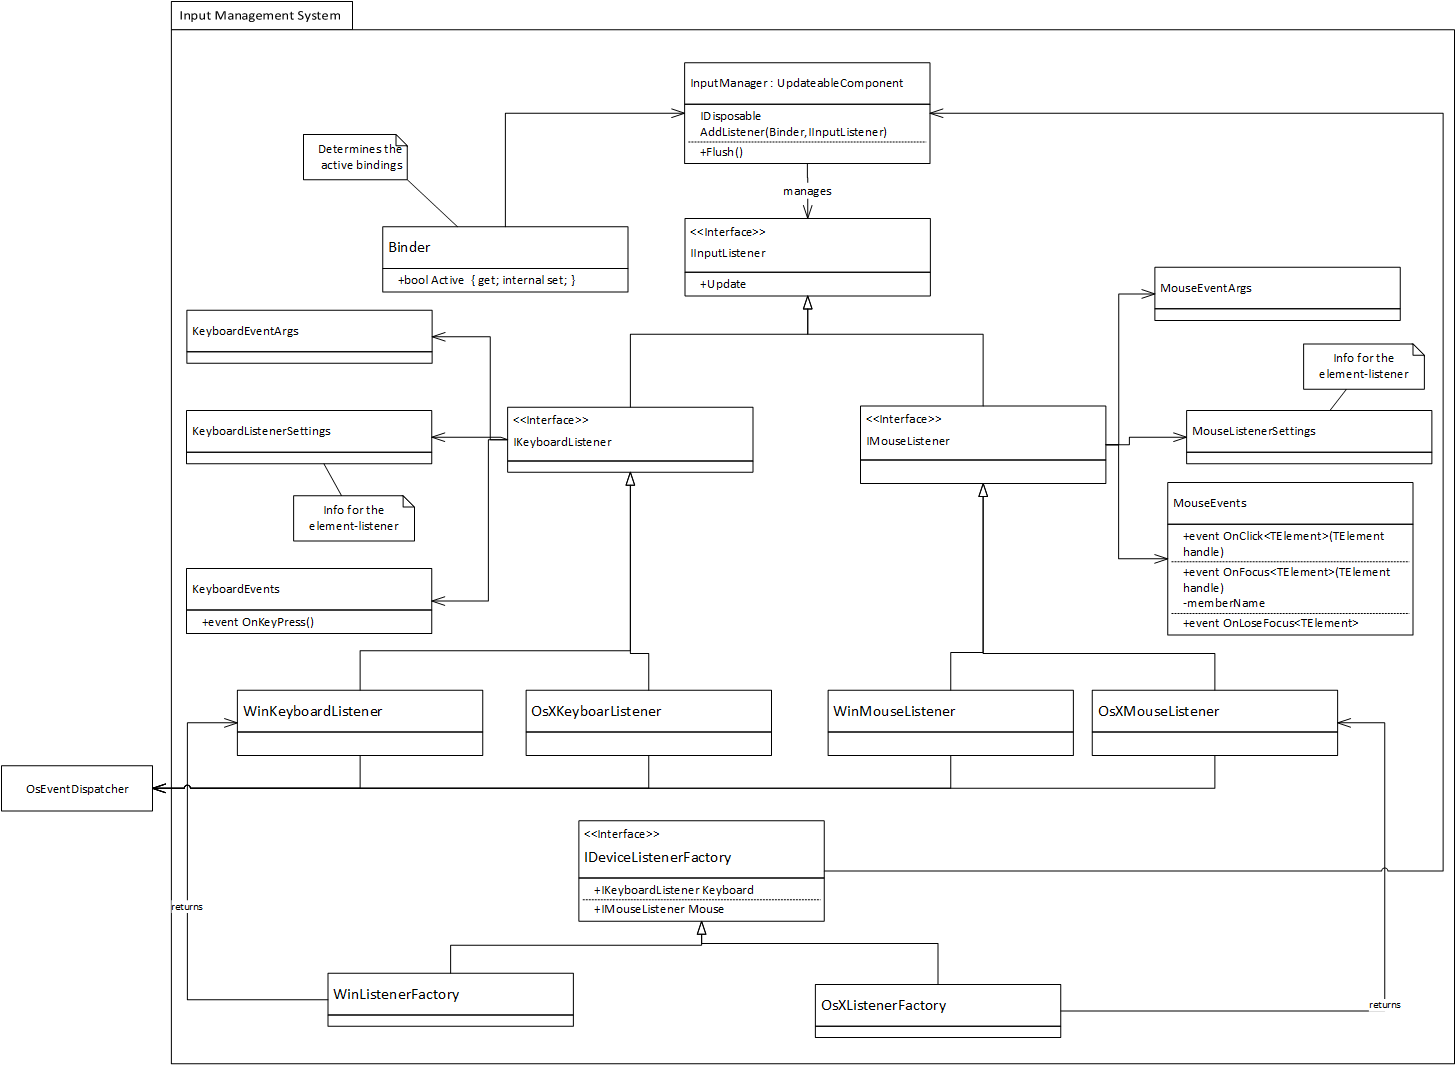
\includegraphics[width=165mm]{Images/core_input}
		\caption{core input architecture}
		\label{fig:core_input}
	\end{figure}
		
	\lstset
	{
		style=sharpc, 
		caption={Παράδειγμα listener στο initialization}
	}
	\begin{lstlisting}
inputManager.AddListener(
ingameBinder,
factory => factory.GamepadListener
{
	Settings = MouseSettings
		    .DoubleClickDelta(Timespan.FromSeconds(0.2))
			.DragDelta(Timespan.FromSeconds(0.2)),
	Events   = MouseEvents
	        .OnLeftClick(sender,args) => this.Shoot())
	        .OnLeftDoubleClick(sender,args) => this.Roll())      	
});

inputManager.AddListener(
ingameBinder,
factory => factory.GamepadListener
{
	Settings = GamepadSettings.Default,
	Events   = GamepadEvents
			.OnXButtonPress(sender,args) => this.Shoot())
			.OnYButtonPress(sender,args) => this.Roll())      	
});
\end{lstlisting}

\section{Physics}
Η φυσική στα παιχνίδια έχουν ως βάση τα μαθηματικά. Η ανάλυση του συστήματος της φυσικής επικεντρώνεται σε μοντελοποίηση υψηλού επιπέδου. Η υλοποίησή τους βασίζεται υλοποίηση μαθηματικών λειτουργιών γεωμετρίας, γραμμικής άλγεβρας και κινηματικής.

\subsection{Τα παιχνίδια ως soft real-time simulations}
Οι επιστήμονες αποκαλούν τα παιχνίδια soft real-time interative agent-based computer simulations.
Στα περισσότερα παιχνίδια ένα υποσύστημα του πραγματικού κόσμου μοντελοποιείται μαθηματικά, ώστε να μπορεί να αναπαραχθεί και να χειριστεί από τον υπολογιστή. 
Ενα agent-based simulation είναι μια προσομοίωση η οποία περιγράφει πως αλληλεπιδρούν τα διάφορα αντικείμενα και χαρακτήρες μέσα στον κόσμο.
Όλα τα αλληλεπιδραστηκά παιχνίδια είναι temporal simulations δηλαδή ο το μοντέλο του εικονικού κόσμου είναι δυναμικό, αλλάζει με την πάροδο του χρόνου, με βάση τα διάφορα συμβάντα και την εξέλιξη της ιστορίας.
Όλα simulations και η επικοινωνία του παιχνιδιού με τον χρήστη γίνεται σε πραγματικό χρόνο (interactive real-time simulations. 

Στον πυρήνα όλων τον συστημάτων πραγματικού χρόνου υπάρχει το at least 24 fps deadline δηλαδή για να δημιουργείται η ψευδαίσθηση της κίνησης, η οθόνη θα πρέπει να ανανεώνεται τουλάχιστον 24 φορές το δευτερόλεπτο. Φυσικά υπάρχουν και άλλα είδη deadlines. Για να θεωρείται η προσομοίωση φυσικής σταθερή, πρέπει να ενημερώνεται τουλάχιστον 120 φορές το δευτερόλεπτο, ο μηχανισμός τεχνητής νοημοσύνης θα πρέπει να καλείται τουλάχιστον κάθε δευτερόλεπτο, οι audio buffers 60 φορές το δευτερόλεπτο για να αποτρέπονται δυσλειτουργίες του συστήματος διαχείρησης ήχου.

Ένα soft real time system είναι ένα σύστημα στο οποίο χαμένες ενημερώσεις δεν είναι καταστροφικές.
Τα μαθηματικά μοντέλα τα οποία απαρτίζουν το σύστημα μπορεί να είναι είτε αριθμητικά είτε αναλυτικά. Τα αριθμητικά μοντέλα μπορούν να αξιολογηθούν για κάθε τιμή της ανεξάρτητης μεταβλητής ενώ οι τιμές του αναλυτικού μοντέλου καθορίζονται διακρίτα κατά τη διάρκεια της προσομείωσης και είναι πιο συχνά γιατί η επόμενη κατάσταση της προσομείωσης καθορίζεται από την εισαγωγή δεδομένων σε πραγματικό χρόνο από το χρήστη.

\subsection{Βασικές έννοιες φυσικής του συστήματος}
Οι οντότητες της φύσικης έχουν τις παρακάτω ιδιότητες για τη προσομοίωσή τους στο υποσύστημα φυσικής.

\begin{itemize}
\item Mass: Η μάζα στη φυσική συνδέεται με δύο έννοιες, την αδράνεια της μεταφορικής κίνησης και τη βαρύτητα. Η μάζα είναι μια ορισμένη ποσότητα η οποία χρησιμοποιείται για την περιγραφή ενός συστήματος.

\item Density:  Η πυκνότητα εκφράζει τη μάζα του υλικου που περιέχεται σε μία μονάδα όγκου. 

\item Force: Σε ότι αφορά τα ελεύθερα σώματα, η δύναμη είναι γενικά η αιτία μεταβολής της κινητικής τους κατάστασης, δηλαδή αυτή που τα επιταχύνει ή τα επιβραδύνει. Αυτό ισχύει και για την περιστροφή τους, που μπορεί να επιταχυνθεί ή να επιβραδυνθεί. Για σώματα που δεν είναι ελεύθερα να κινηθούν με όλους τους τρόπους, αυτά δηλαδή που είτε είναι αναρτημένα κάπου και μπορούν να κινηθούν μόνο γύρω από σημείο ή άξονα ή σε προκαθορισμένη τροχιά, καθώς και σε όσα εφαρμόζονται δυνάμεις τριβής ή γενικά αντιδράσεις στήριξης.

\item Torque: Ροπή δυνάμεως ως προς σημείο είναι το διανυσματικό φυσικό μέγεθος που έχει μέτρο ίσο προς το γινόμενο της δύναμης επί την (κάθετη) απόσταση της δύναμης από το σημείο. Κατά όμοιο τρόπο ροπή δυνάμεως ως προς άξονα είναι το διανυσματικό μέγεθος που έχει ως μέτρο το γινόμενο της δύναμης επί την (κάθετη) απόσταση της δύναμης από τον άξονα, και φορέα τον άξονα.

\item Impulse: Η ώθηση είναι φυσικό μέγεθος που ισοδυναμεί με την μεταβολή της ορμής ενός σώματος στο οποίο εφαρμόζεται μία δύναμη για κάποιο χρονικό διάστημα. Ισούται με το γινόμενο της δύναμης που ασκείται στο σώμα επί τον συνολικό χρόνο εφαρμογής της

\item Restitution: Το law of restitution δηλαδή ανάκτυση με βάση το κέρδος. Η υποχρέωση της οντότητας να αποζημιώσει από τα κέρδη τη για κάποιο γεγονός. 

\item Damping: Η απόσβεση, η επιρροή εντός η κατά ενός συστήματος ταλάντωσης που έχει ως αποτέλεσμα τη μείωση, τον περιορισμό η την πρόληψη των ταλαντώσεών του. Σε φυσικά συστήματα , απόσβεση παράγεται με διαδικασίες που διαχέουν την ενέργεια που αποθηκεύεται στο ταλάντωση.
\end{itemize}

\subsection{Οντότητες του συστήματος}
\begin{itemize}
\item Shape
Ένα αντικείμενο το οποίο αντιπροσωπεύει ένα γεωμετρικό σχήμα όπως κύκλο, πολύγωνο κλπ
\item World
Η συλλογή των bodies, fixtures και constraints και η λογική της αλληλεπίδρασής τους.
\item World Solver
Ο solver αναλύει την προσομοίωση και εκτελείται ανεξάρτητα από το χρόνο εκτέλεσης του προγράμματος.
\item Fixture 
To fixture δένει ένα body με ένα shape και προσθέτει επιπλέον ιδιότητες όπως πυκνότητα, τριβή και αποκατάσταση. Το fixture εντάσσει ένα σχήμα στο σύστημα συγκρούσεων ώστε να αλληλεπιδρά με τα υπόλοιπα σχήματα στον κόσμο.
\item Body 
To body περιέχει της πληροφορίες ένος αντικειμένου του οποίου δεν βλέπεις ούτε συγκρούεσαι. Έχουν τις παρακάτω ιδιότητες
	\begin{itemize}
		\item mass To βάρος
		\item velocity η ταχύτητα και η κατεύθυνση της κίνησης υπό μορφή διανύσματος.
		\item rotation inertia πόσος κόπος χρειάζεται για να ξεκίνησει η περιστροφή ή η κίνηση
		\item angular velocity πόσο γρήγορα και σε ποια κατεύθυνση περιστρέφεται
		\item που βρίσκεται στο σύστημα καρτεσιανών συντεταγμένων
		\item angle υπό ποια γωνία βρίσκεται
	\end{itemize}
Οι τύποι των bodies είναι:
	\begin{itemize}
		\item Static
		Στατικά στο σύστημα συντεταγμένων. Δεν ανταποκρίνεται σε εξωτερικές δυνάμεις.
		\item Dynamic
		Είναι μέρος του συστήματος συγκρούσεων. Ανταποκρίνεται σε εξωτερικές δυνάμεις και κανονικά σε όλες τα μέρη της προσωμοίωσης.
		\item Kinematic 
		Κινείται ανάλογα με το προκαθορισμένο script ταχύτητας. Δεν ανταποκρίνεται σε εξωτερικές δυνάμεις.
	\end{itemize}
\item Constraint
Περιορισμός κατά την προσωμοίωση του body.
\item Joint 
Το joint συνδέει δύο ή περισσότερα bodies μεταξύ τους.
\item Joint Motor
Ο οδηγός της κίνησης των συνδεδεμένων με joint bodies. 
\item Joint Limit
Περιορίζει το εύρος κίνησης του joint motor.
\end{itemize}

\subsection{Αρχιτεκτονική}
	\begin{figure}[h!]
		\centering
		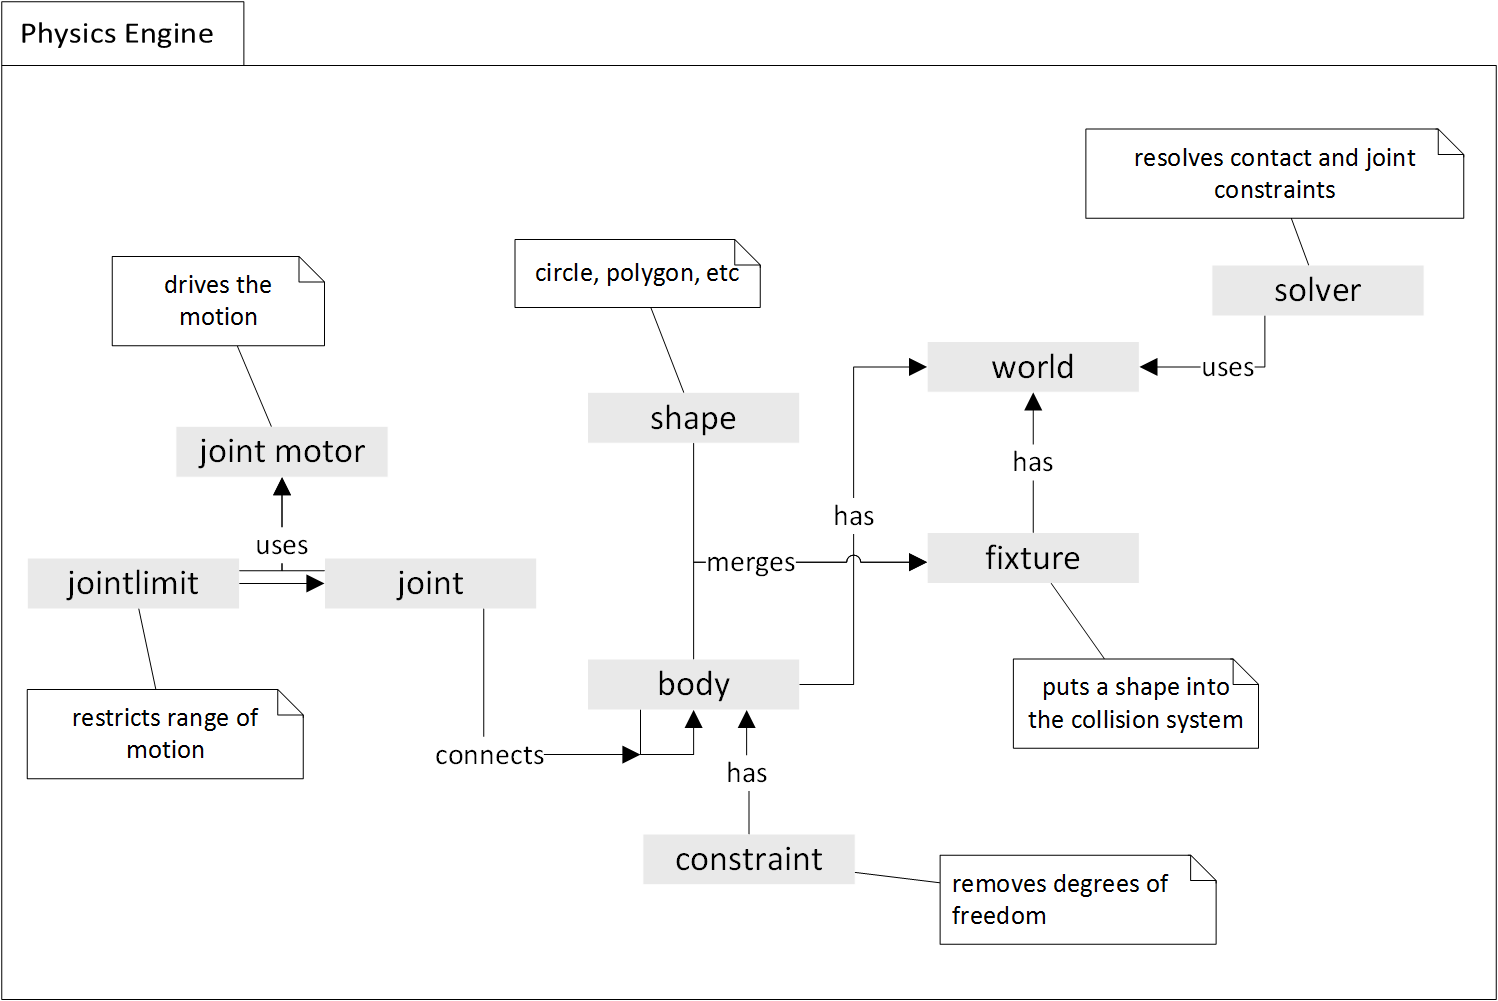
\includegraphics[width=165mm]{Images/physics_overview}
		\caption{Physics Architecture Abstract}
		\label{fig:physics abstract}
	\end{figure}
	
\section{UI}
Η επικοινωνία του χρήστη με τη μηχανή γίνεται συνήθως με human interface devcices. Η επικοινωνία αυτή αντί να περιορίζεται σε ένα απλό input signal, μπορεί να γίνει εύκολα, αυτονόητα, αποτελεσματικα και φιλικά προς το χρήστη. Το User interface (διεπαφή χρήστη) ονομάζουμε το σύνολο γραφικών στοιχείων, τα οποία εμφανίζονται στην οθόνη κάποιας ψηφιακής συσκευής (π.χ. Η/Υ) και χρησιμοποιούνται για την αλληλεπίδραση του χρήστη με τη συσκευή αυτή. Παρέχει μέσω γραφικών ενδείξεις και εργαλεία προκειμένου ο χρήστης να φέρει εις πέρας κάποιες επιθυμητές λειτουργίες.

\subsection{Απαιτήσεις}
Κατά το σχεδιασμό ενώς παιχνιδίου συχνά δημιουργείται η ανάγκη για διεπαφή χρήστη. Η δομή του UI, το στυλ της απόδοσης (χρώμα, textures, fonts κλπ),η απόδοσης (rendering) και η συμπεριφορά και ο εκτελέσιμος κώδικας κατά τα συμβάντα της διεπαφής πρέπει να είναι αποσυνδεδεμένα έτσι ώστε να μην επηρεάζει το ένα το άλλο. Επίσης χρησιμεύει όταν το UI προορίζεται για διάφορες αναλύσεις και \Gls{DPI}. Μια καλή στρατηγική σστην κατανόηση και επίλυση προβλημάτων είναι η εύρεση παρόμοιων και σχετικών προβλημάτων. Στο σχεδιασμό ιστοσελίδων η HTML χρησιμοποιείται και τη δομή της σελίδας, το CSS για το στυλ και η Javascript για τη συμπεριφορά.

\subsection{Δομή στη μνήμη}	
Όταν ζητηθεί από τον περιηγητή να φορτώσει μια ιστοσελίδα στη μνήμη από κάποιον web server, αναλύει το html αρχειο και οργανώνει τα στοιχεία σε δομή δέντρου \gls{B-Tree}. Λόγω της οργάνωση σε δέντρο, δημιουργούνται σχέσεις μεταξύ των στοιχείων, 

	\begin{figure}[h!]
		\centering
		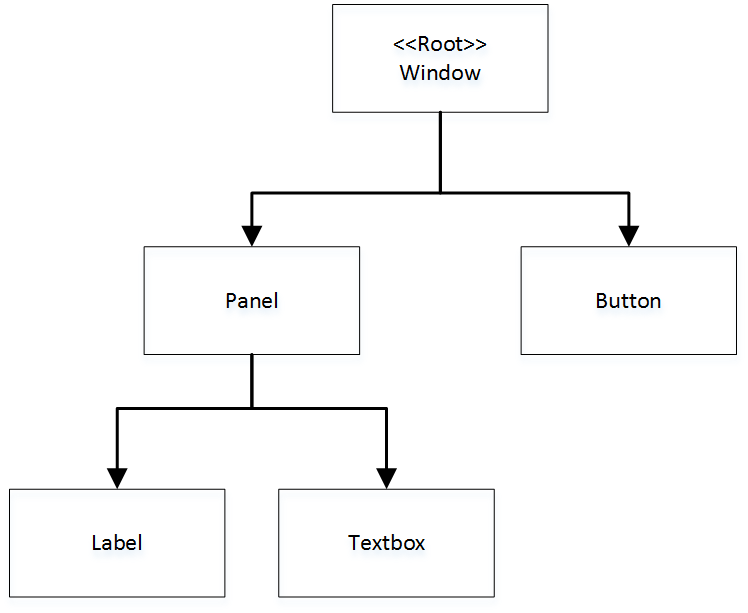
\includegraphics[width=90mm]{Images/ui_btree}
		\caption{UI B-Tree}
		\label{fig:ui_b-tree}
	\end{figure}
	
Στο παράδειγμα \ref{fig:ui_b-tree}  το window είναι το root του δέντρου. Το window έχει δύο παιδιά, ένα panel και ένα button. Το button έχει με και αυτό δύο παιδιά: ένα textbox και ένα label. Τα button, textbox και label είναι leafs του δέντρου, το panel είναι node, και το panel και button siblings.

\paragraph{Γιατί b-tree;}
Η οργάνωση σε b-tree έχει τα παρακάτω πλεονεκτήματα.
\begin{itemize}
	\item Ευκολία κατά την απόδοση στην οθόνη. Λόγω της συγκεκριμένης δομή, τα στοιχεία μπορούν να στοιχιθούν και να αποδοθούν ανάλογα με τη σχέση τους με συγγενικά στοιχεία. Καθώς διαβαίνεται το δεντρο, το κάθε στοιχείο αποδίδεται μέσα στο πλαίσιο του πατέρα του και σε πιο πάνω επίπεδο, ούτως ώστε να δημιουργείται η ψευδαίσθηση του βάθους, δηλαδή ότι το στοιχείο παιδί βρίσκεται "πάνω" άπο τον πατέρα.
	\item Καλύτερη απόδοση στο rendering. Όταν κάποιος κόμβος δεν διατέμνεται με το πλάισιο του παράθυρου, δεν απόδίδεται στην οθόνη και το traversing του δέντρου σταματά.
	\item Αποσαφήνιση σειράς συμβάντον. Κατά τα συμβάντα στο UI, ένα πλαίσιο μπορεί να καλύπτει περισσότερα από ένα συμβάντα. Ένα στοιχείο έχει τεμνόμενα πλαίσια όταν οποίο βρίσκεται μέσα σε ένα άλλο στοιχείο. To συμβάν γίνεται στο στοιχείο το οποίο βρίσκεται τελευταίο στην ιεραρχία.
	\item Προχωρημένη και γρήγορη επιλογή στοιχείων. Η επιλογή των στοιχείων γίνεται με προχωρημένα κριτήρια, όπως τη σχέση ενός στοιχείου με συγγενικά στοιχεία στη δομή, και σε λογαριθμηκό χρόνο.
\end{itemize}
	\begin{figure}[h!]
		\centering
		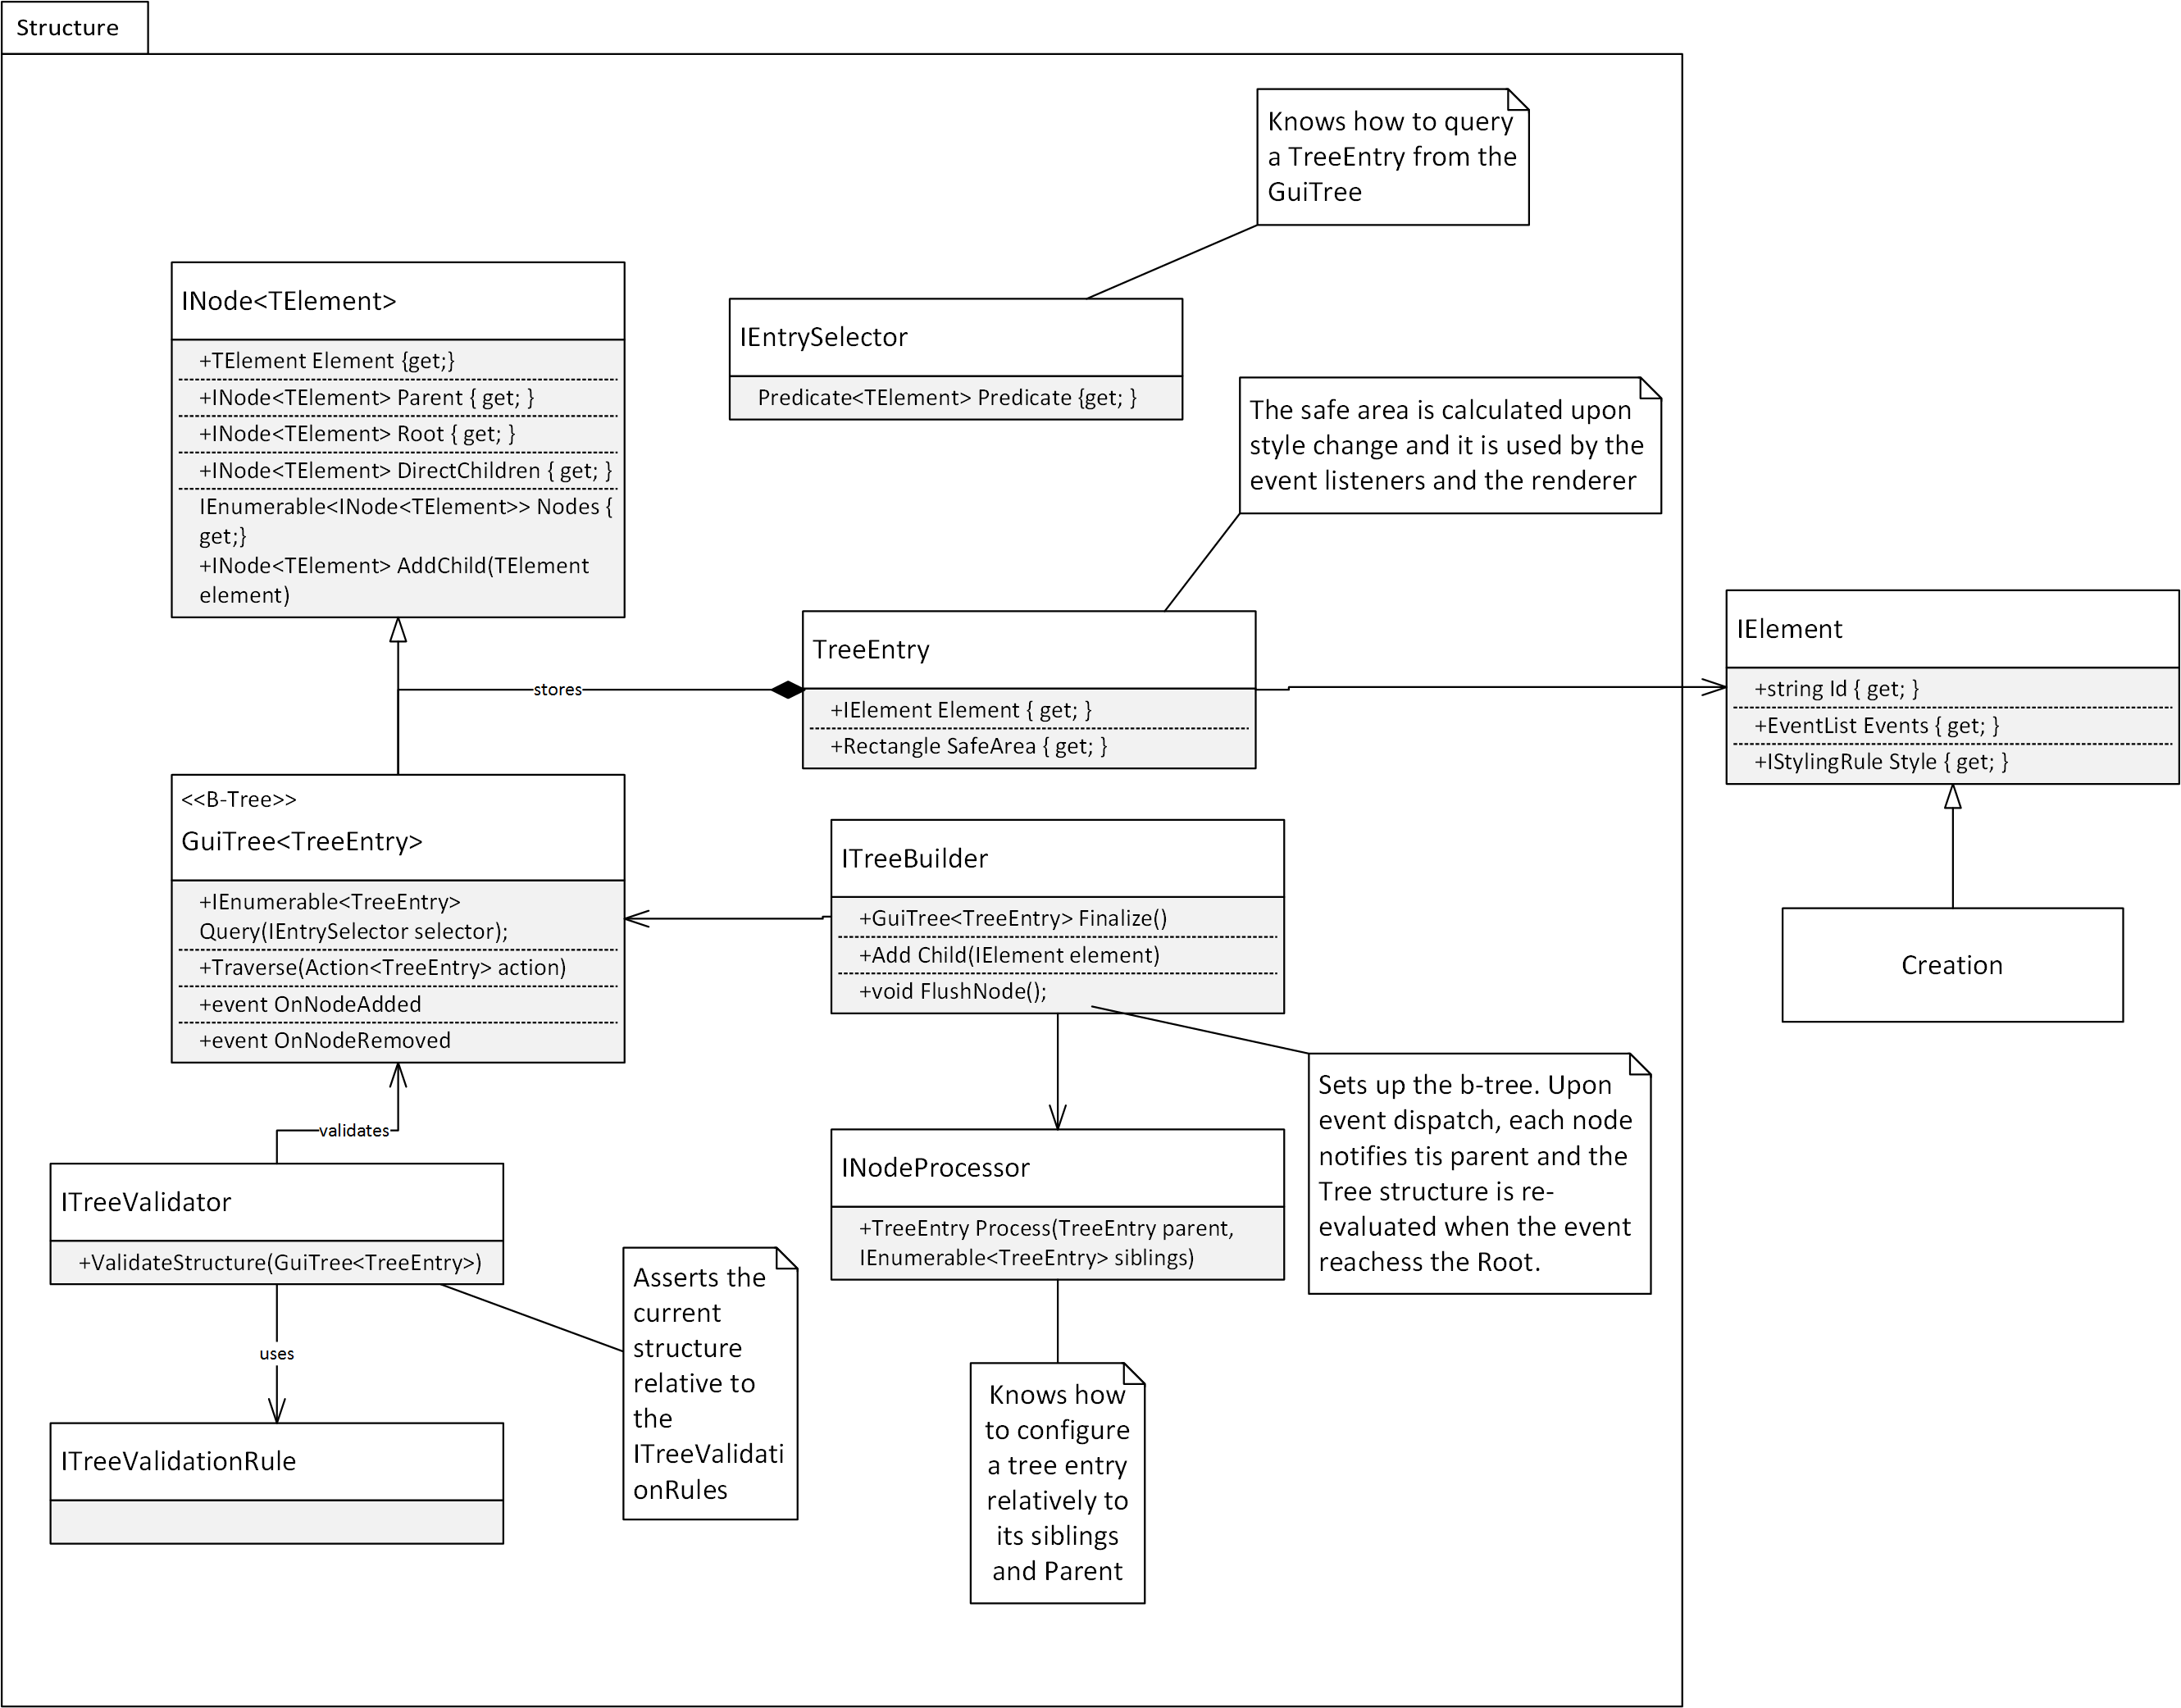
\includegraphics[width=165mm]{Images/gui_structure}
		\caption{Gui Structure Diagram}
		\label{fig:gui_structure}
	\end{figure}

\subsection{Το σύστημα}	
Το σύστημα ανθρώπινης διεπαφής χωρίζεται στα παρακάτω υποσυστήματα
	\begin{itemize}
		\item Οργάνωσης δομής, το οποίο κτίζει και αποθηκεύει την ιεραρχία τον στοιχείων στη μνήμη
		\item Style definition το οποίο επαυξάνει την απόδοση με animations, textures κλπ
		\item Factory μέσα από το οποίο ο χρήστης δημιουργεί στοιχεία. Στο υποσύστημα αυτό, όπως και το input listener factory είναι χρησιμοποιεί abstract factory για δημιουργεία στοιχείων ανεξαρτήτου πλατφόρμας, και fluent builder για τη δημιουργία στοιχείων με φιλικό στον χρήστη \gls{API}.
		\item Επεκτίνει και χρησιμοποιεί με το input system για να συνδέει συμβάντα με στοιχεία
		\item Επεκτίνει και χρησιμοποιεί το rendering module για να αποδίδει το δεντρο στην οθόνη.
	\end{itemize}
	\begin{figure}[h!]
		\centering
		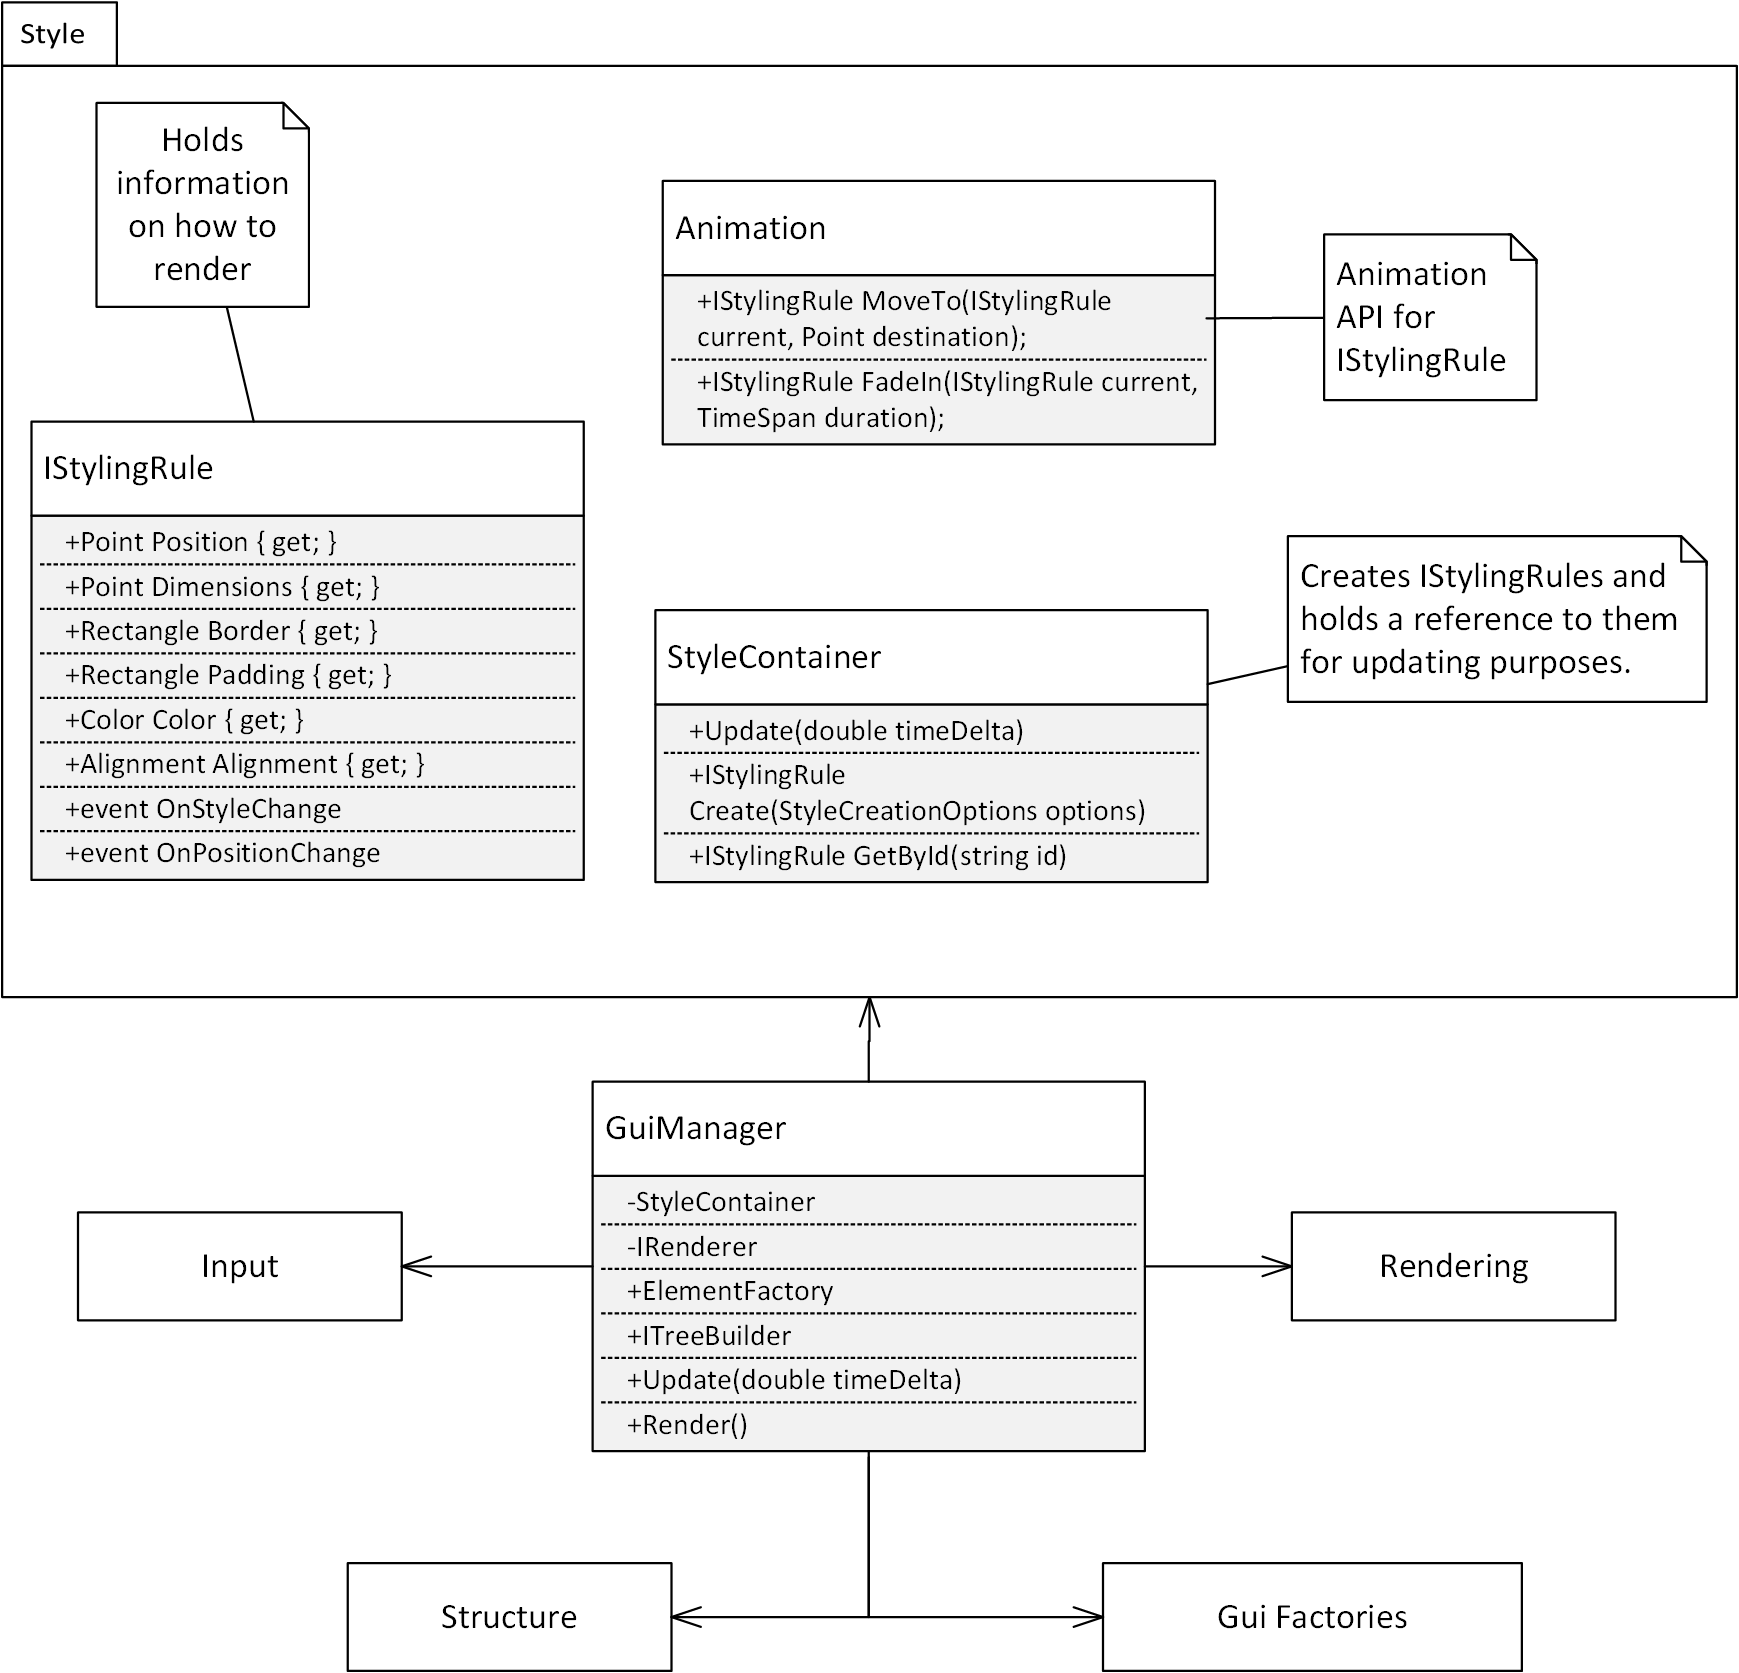
\includegraphics[width=165mm]{Images/gui_system}
		\caption{Gui System Diagram}
		\label{fig:gui_system}
	\end{figure}	

\subsection{Τρόπος χρήσης}
Usage pipeline
\begin{figure}[h!]
	\centering
	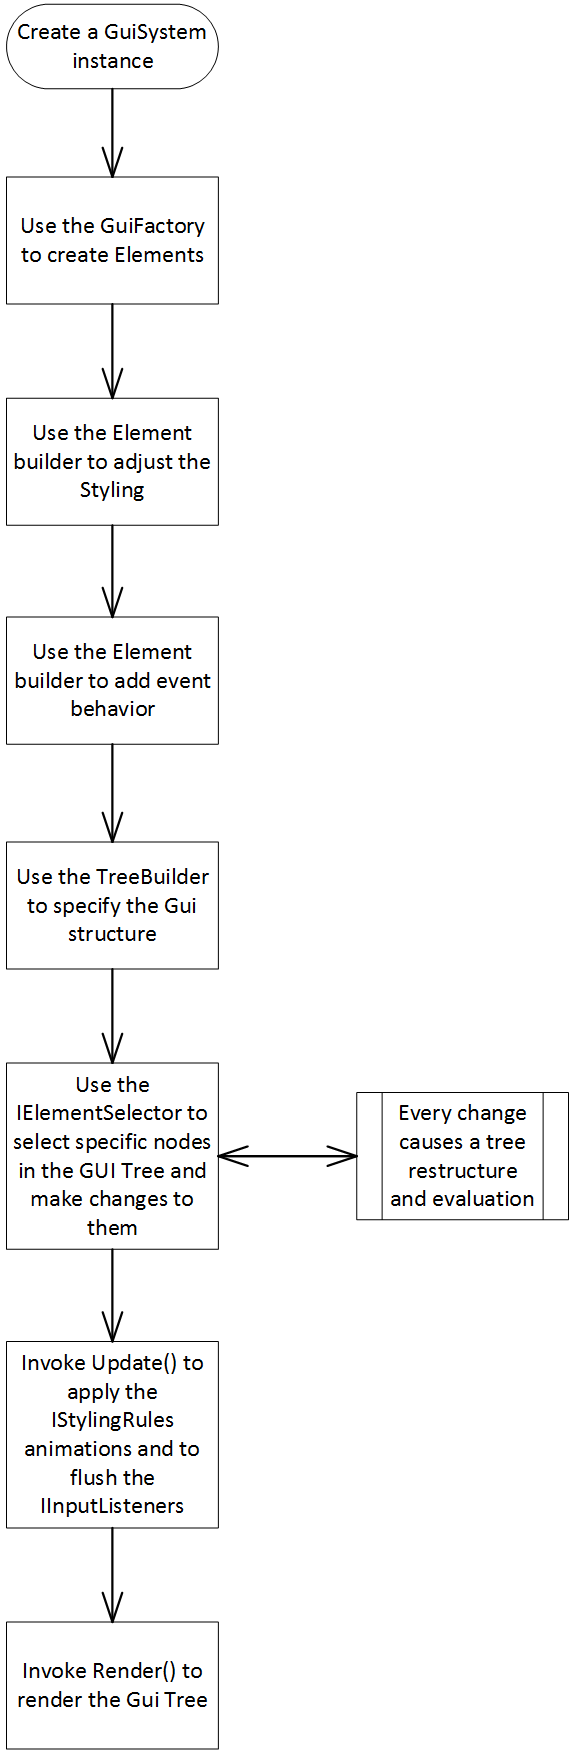
\includegraphics[width=80mm]{Images/gui_usage}
	\caption{Gui Usage Diagram}
	\label{fig:gui_usage}
\end{figure}

\section{Resource Management}
Τα παιχνίδια απαρτίζονται από πολλα είδη δεδομένων, είτε αυτά είναι τρισδιάστατα μοντελα, είτε είναι textures είτε αρχεία ήχου κλπ. Η μηχανή πρέπει να είναι σε θέση να φορτώνει στη μνήμη και να αφαιρεί αυτά τα δεδομένα δυναμικά. Χρειάζεται λοιπόν κάποιου είδους asset / resource manager, ο οποίος χειρίζεται το σύστημα αρχείων του λειτουργικού. Ο asset manager πρέπει να προσαρμόζεται ανάλογα με το λειτουργικό στο οποίο τρέχει και να λαμβάνει υπόψη τις ιδιαιτερότητες των διάφορων συστημάτων αρχείων. Πρέπει να υποστηρίζεται το ασύγχρονο φόρτωμα δεδομένων, για να μην μπλοκάρεται η ροή του παιχνιδιού.

Ο resource manager απαρτίζεται από δύο μέρη. Το πρώτο χειρίζεται εργαλεία τα οποία χειρίζονται assets και τα μεταφράζουν σε μια μορφή η οποία είναι επεξεργάσιμη από τη μηχανή. Το δεύτερο διαχειρίζεται τα assets, φροντίζει να είναι διαθέσιμα όταν χρειάζονται  και όταν δεν θα ξαναχρησιμοποιηθούν φροντίζει να αφαιρέσει από τη μνήμη.
Τα περισσότερα assets δεν φορτώνονται στη μνήμη με την κανονική τους μορφή. Τα assets περνούν από κάποιο conditioning pipeline για να μετασχηματιστούν σε ένα format το οποίο μπορεί να επεξεργαστεί η μηχανή. Δεν είναι αρκετό απλά ένα μοντέλο, η μηχανή πρέπει να ξέρει για τι προορίζεται. Περιέχουν metadata το οποίο περιγράφει το πως η μηχανή θα χειριστεί το συγκεκριμένο asset. 
Χρειάζεται μια resource database η οποία ξέρει πως να χειρίζεται διάφορα είδη assets σε μια μορφή την οποία η μηχανή καταλαβαίνει. Μπορεί απλά το κάθε asset να περιέχει μαζί του κάποιο αρχείο xml το οποίο εξηγεί τι θα κάνει η μηχανή μαζί του. Επίσης είναι χρήσιμο να υποστηρίζει  versioning. Η βάση μπορεί να είναι είτε SQL είτε απλά ένα b-tree με buffer blocks και δυνατότητα προσπέλασής του. 

\paragraph{Σχεδιασμός Resource Pipeline}
\begin{itemize}
\item Granular resoures:  resources τα οποία συνδέονται με τις οντότητες στο παιχνίδι. 
\item Συνδεση με κώδικα: μπορεί εύκολα να γίνει η σύνδεση των δεδομένων με τον πηγαίο κώδικα
\item Ευκόλo export δεδομένων σε διάφορα formats.
\item Συμβατότητα με άλλα formats ή δυνατότητα μετατροπής τους σε format το οποίο είναι συμβατό με τη μηχανή.
\item Εύκολο build, αφού η μηχανή αναλαμβάνει τις εξαρτήσεις μεταξύ δεδομένων και κώδικα.
\end{itemize}

\subsection{Ευθύνες του offline resource manager}
\begin{itemize}
\item Exporters η δυνατότητα μετατροπής native format σε format το οποίο μπορεί να τροποποιηθεί από τη μηχανή.
\item Resource Compilers κατά το export χρειάζεται να γίνει κάποιου είδους καμουφλάρισμα των δεδομένων ώστε να συμβαδίζουν με την μηχανή.
\item Resource Linkers πολλές φορές περισσότερα από ένα αρχεία χρειάζονται να συνδεθούν για να δημιουργηθεί ένα χρήσιμο πακέτο. Η είναι υπεύθυνη στο να βρίσκει εξαρτήσεις και να ενώνει κομμάτια ώστε να δημιουργεί πακέτα έτοιμα χρησιμοποιηθούν.
\end{itemize}

\subsection{Ευθύνες του Runtime- Resource Manager}
\begin{itemize}
\item Εξασφαλίζει ότι στη μνήμη υπάρχουν μόνο μοναδικά resources και περισσότερα από ένα του ίδιου τύπου.
\item Διαχειρίζεται το πόσο χρόνο είναι διαθέσημα στη μνήμη
Φορτώνει και ξεφορτώνει απο τη μνήμη
\item Χειρίζεται composite resources δηλαδή resource το οποίο αποτελείται από περισσότερες από μία. Ένα τρισδιάστατο μοντέλο για παράδειγμα, αποτελείται από ένα mesh, materials, textures, skeletal animations κλπ
\item Διαχειρίζεται την ακεραιότητα των αναφορών, δηλαδή λαμβάνει υπόψη τις υποεξαρτίσεις και τις αλληλοεξαρτίζεις και φροντίζει να μην υπάρχουν προβλήματα.
\item Διαχειριση μνήμης.
\item Επιστρέπει την τροποποίηση των δεδομένων αφού φορτωθούν στη μνήμη
\item Προσφέρει τη δυνατότητα ασύγχρονης φόρτωσης για παραλλελησμό ενεργειών.
\end{itemize}

\paragraph{Οργάνωση αρχείων και καταλόγων}
Συνήθως γίνεται δενδροειδής οργάνωση για τα resources.  Πολλές φορές για σκοπούς επίδοσης, πολλά αρχεία είναι συμπιεσμένα σε ένα για να γινέται πιο γρήγορη προσπέλαση. Μια μηχανή μπορεί να χρησιμοποιήσει ήδη υπάρχων formats ή κάποιο προσαρμοσμένο για τις ανάγκες της μηχανής. 

\paragraph{Τεχνικές διαχείρισης resources στη μνήμη}
Μια συνηθισμένη τεχνική είναι η οργάνωση σε δομή δεδομένων hashtable με κλειδιά και τιμές, όπου κλειδί είναι το μοναδικό χαρακτηριστικό, ένα GUID ή η διαδρομή του αρχείου στο δίσκο. (flyweight pattern). Όταν το παιχνίδι χρειάζεται κάποιο resource, η μηχανή ελέγχει αν υπάρχει το κλειδί. Αν υπάρχει τό επιστρέφει και αν όχι τότε φορτωνεί στο hashtable.

\paragraph{Διαχείριση του κύκλου ζωής στη μνήμη}
\begin{itemize}
\item Global resources: κάποια resources φορτώνονται στην αρχή του παιχνιδιού και χρειάζονται συνέχεια.
\item Level resources: άλλα χρειάζονται στο scope συγκεκριμένου level-layout
\item Short-living resources: κάποια χρειάζονται για ένα συγκεκριμένο σκοπό κατα τι διάρκεια π.χ. μια σκηνή η οποία εμφανίζεται μια φορά κατα τη διάρκεια ενός level.
\item Live streamed resources: αρχεία μουσική και ηχητικών εφέ τα οποία διαβάζονται από το δίσκο δυναμικά και φορτώνονται σε chunks.
\end{itemize}

\paragraph{Τεχνκές διαχείρισης κύκλου ζωής}
Υπάρχουν διάφορες τεχνικές για τη διαχείρηση του κύκλου ζωής των resources. Μια καλή τεχνική είναι να φυλάονται τα references στα αντικείμενα κάθε φορά που γίνεται προσπέλαση στη μνήμη π.χ. στην αρχή κάθε level.
Μετράται πόσες φορές ζητήθηκε συγκεριμένο resource.  
Βημα 1: Βρίσκουμε όλα τα resources που χρειάζονται για τη συγκεκριμένη σκηνή και αυξάνουμε τον μετρητή τους κατά 1. Αφαιρούμε στα υπόλοιπα 1.
Βήμα 2: Σε όσα ο μετρητής έγινε 1, τα φορτώνουμε στη μνήμη και σε όσα έγινε 0 τα αφαιρούμε από τη μνήμη.

\begin{figure}[h!]
	\centering
	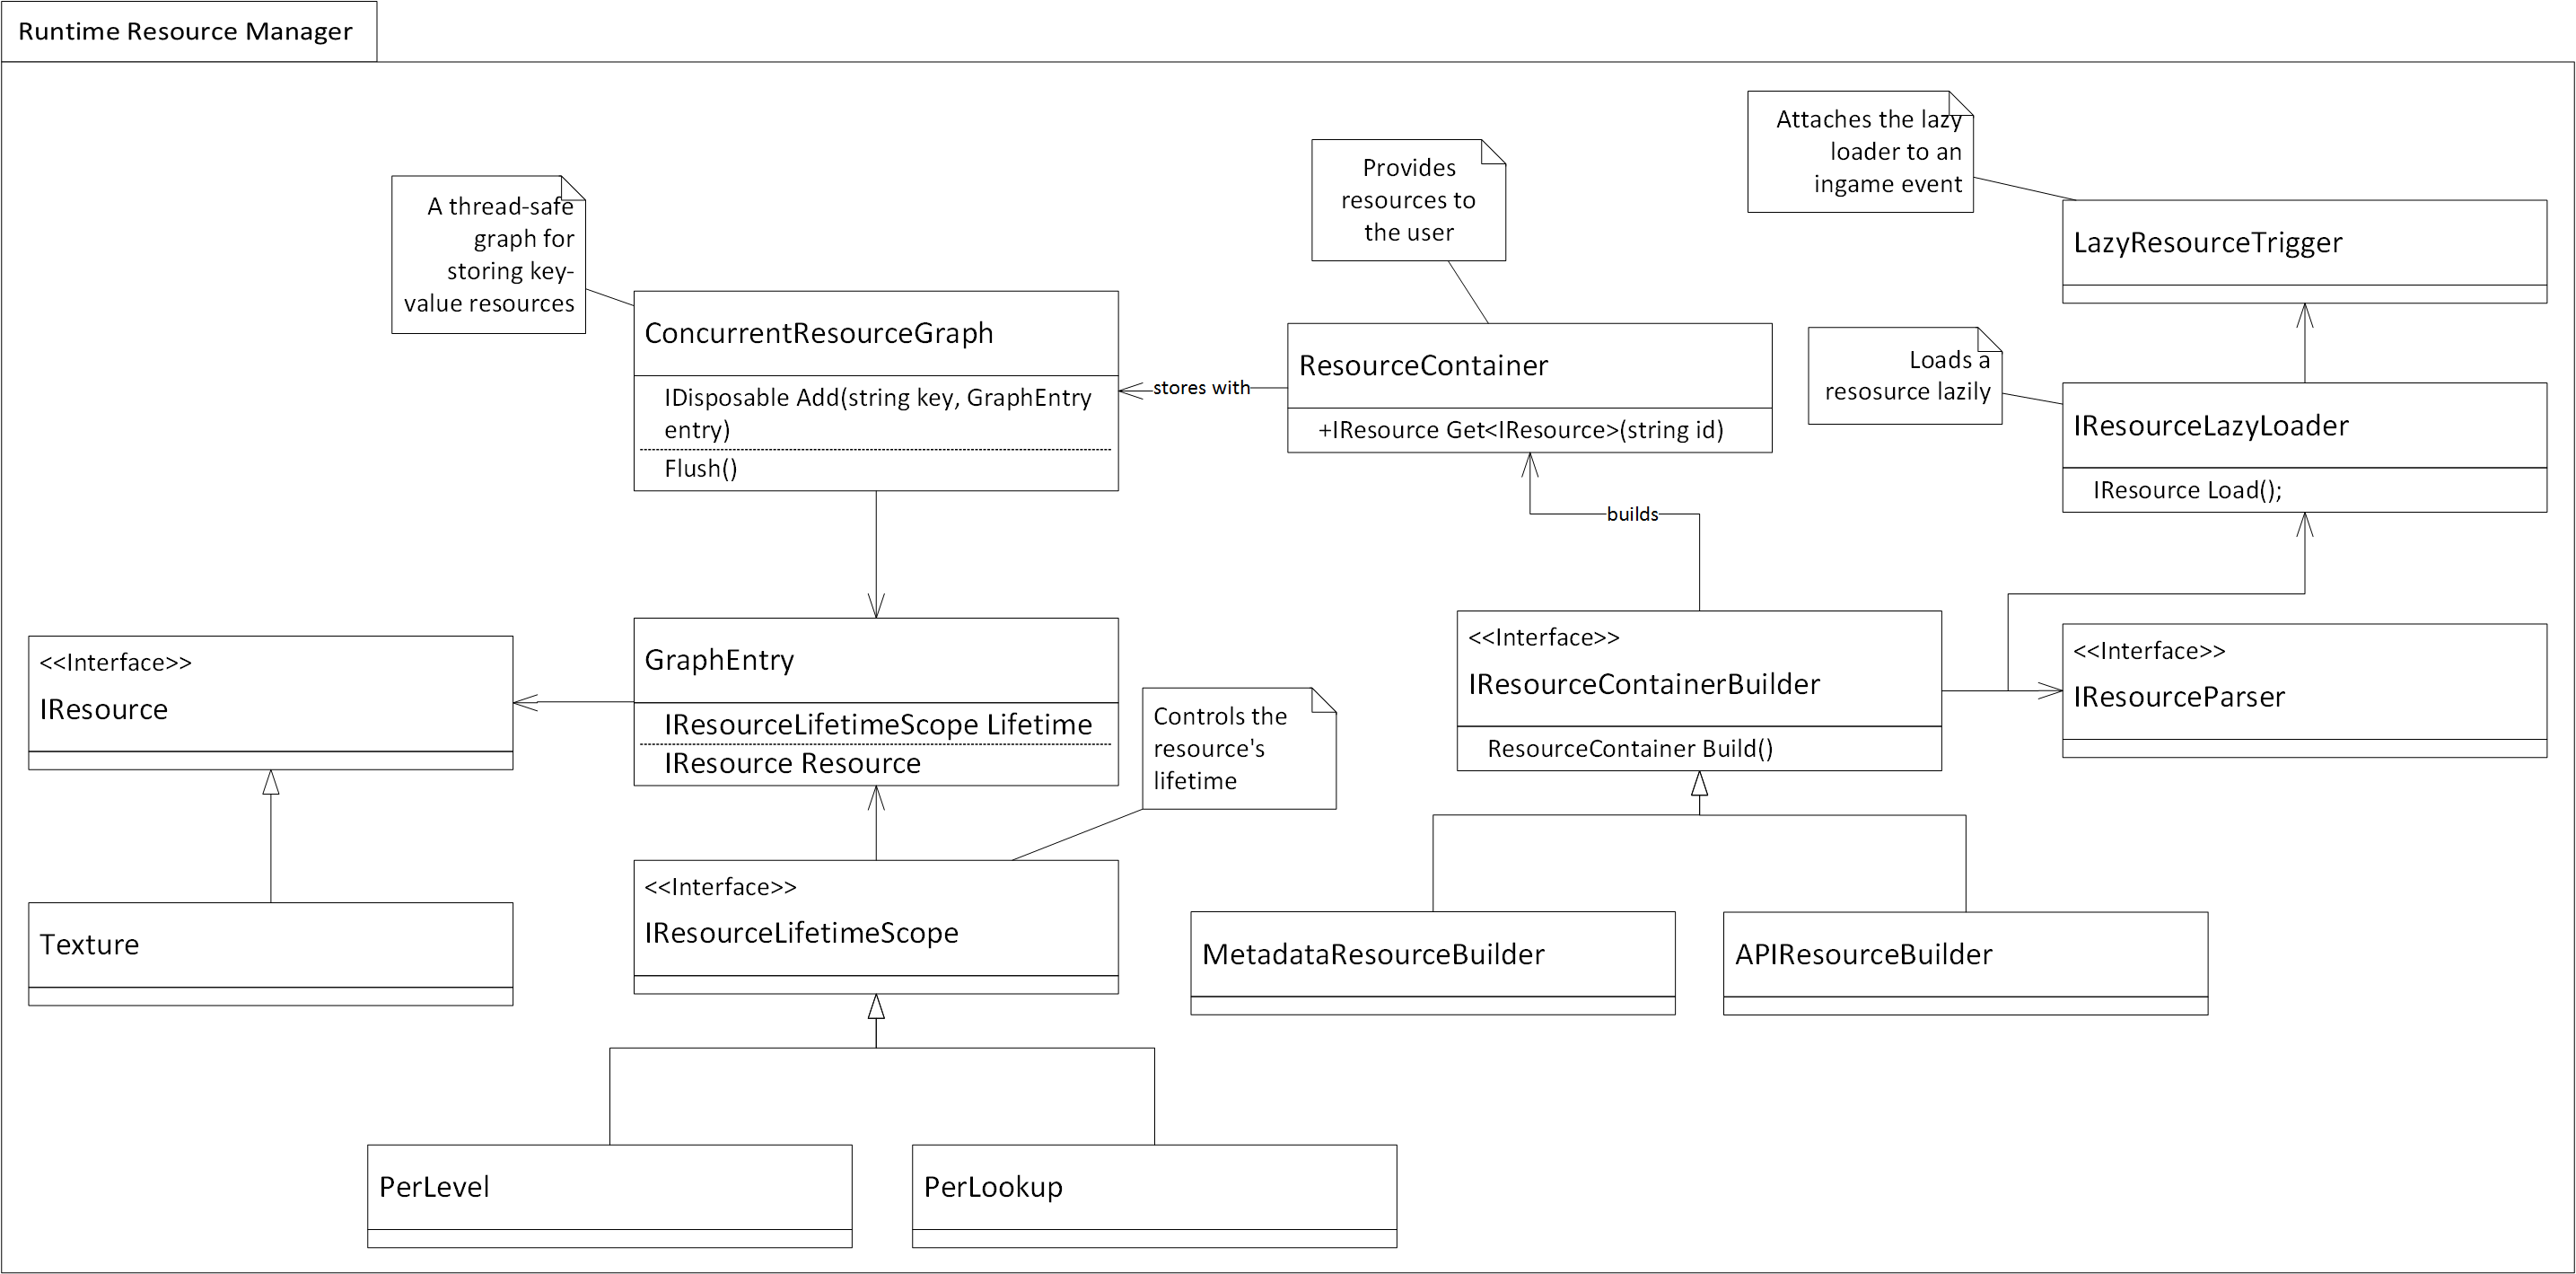
\includegraphics[width=165mm]{Images/runtime_resource_manager}
	\caption{Runtime Resource Manager}
	\label{fig:runtime_resource_manager}
\end{figure}
	